% arara: pdflatex: { synctex: yes }
% arara: makeindex -s ctuthesis.ist -t _main.nlg -o _main.nls _main.nlo
% arara: bibtex
% arara: nomencl
% arara: pdflatex
% makeindex -s ctuthesis.ist _main

% The class takes all the key=value arguments that \ctusetup does,
% and a couple more: draft and oneside
\documentclass[twoside]{ctuthesis}

\ctusetup{
	preprint = \ctuverlog,
%	mainlanguage = english,
	titlelanguage = czech,
	mainlanguage = czech,
	otherlanguages = {slovak,english},
	title-czech = {Tvarová optimalizace lopatkové mříže sdruženou metodou},
	title-english = {Shape optimization of blade cascade with adjoint method},
	subtitle-czech = {},
	subtitle-english = {},
	doctype = M,
	faculty = F2,
	department-czech = {Ústav technické matematiky},
	department-english = {Department of Mathematics},
	author = {Bc. Pavel Mačák},
	supervisor = {doc. Ing. Jiří Fürst, Ph.D.},
	supervisor-address = { Ústav technické matematiky \\ Resslova 307/9 \\ Praha 6},
	%supervisor-specialist = {John Doe},
	fieldofstudy-english = {Mathematical modelling},
	subfieldofstudy-english = {Applied Sciences in Mechanical Engineering},
	fieldofstudy-czech = {Matematické modelování v technice},
	subfieldofstudy-czech = {Aplikované vědy ve strojním inženýrství},
	keywords-czech = {Optimalizace, CFD, OpenFOAM, Lopatková mříž},
	keywords-english = {Optimization, CFD, OpenFOAM, Compressor cascade},
	day = 1,
	month = 1,
	year = 2022,
	specification-file = {others/zadani_BP.pdf},
	front-specification = true,
%	front-list-of-figures = false,
%	front-list-of-tables = false,
%	monochrome = true,
	layout-short = true,
}

\ctuprocess

\addto\ctucaptionsczech{%
	\def\supervisorname{Vedoucí}%
	\def\subfieldofstudyname{Studijní program}%
}

\ctutemplateset{maketitle twocolumn default}{
	\begin{twocolumnfrontmatterpage}
		\ctutemplate{twocolumn.thanks}
		\ctutemplate{twocolumn.declaration}
		\ctutemplate{twocolumn.abstract.in.titlelanguage}
		\ctutemplate{twocolumn.abstract.in.secondlanguage}
		\ctutemplate{twocolumn.tableofcontents}
		\ctutemplate{twocolumn.listoffigures}
	\end{twocolumnfrontmatterpage}
}

% Theorem declarations, this is the reasonable default, anybody can do what they wish.
% If you prefer theorems in italics rather than slanted, use \theoremstyle{plainit}
\theoremstyle{plainit} 
\newtheorem{theorem}{Theorem}[chapter]
\newtheorem{corollary}[theorem]{Corollary}
\newtheorem{lemma}[theorem]{Lemma}
\newtheorem{proposition}[theorem]{Proposition}
\newtheorem{definition}[theorem]{Definice}
\newtheorem{problem}[theorem]{Problém}

\theoremstyle{definition}
\newtheorem{example}[theorem]{Example}
\newtheorem{conjecture}[theorem]{Conjecture}

\theoremstyle{note}
\newtheorem*{remark*}{Remark}
\newtheorem{remark}[theorem]{Remark}

\setlength{\parskip}{5ex plus 0.2ex minus 0.2ex}

\clubpenalty 10000  %prvni radek odstavce nebude sam na konci stranky (vdova) 
\widowpenalty 10000 %posledni radek odstavce nepujde na novou stranku  (sirotek) 


% Abstract in Czech
\begin{abstract-czech}
	\lipsum[1]

\end{abstract-czech}

% Abstract in English
\begin{abstract-english}
	\lipsum[1]

\end{abstract-english}

% Acknowledgements / Podekovani
\begin{thanks}
Chtěl bych poděkovat svému vedoucímu práce doc. Ing. Jiřímu Fürstovi, Ph.D. za odborné vedení, za pomoc a rady při zpracování této práce. Zároveň děkuji své rodině a přátelům za jejich podporu při studiu.
\end{thanks}

% Declaration / Prohlaseni
\begin{declaration}
Prohlašuji, že jsem předloženou práci vypracoval samostatně a uvedl veškerou použitou literaturu.

V Praze, \ctufield{day}.~\monthinlanguage{title}~\ctufield{year}
\end{declaration}

% Only for testing purposes
\listfiles
\usepackage{amsmath, gensymb}
\usepackage[pagewise]{lineno}
\usepackage{lipsum,blindtext}
\usepackage{mathrsfs} % provides \mathscr used in the ridiculous examples
\usepackage{mathtools}

\usepackage{scrextend}

\usepackage[]{nomencl} 
\makenomenclature
\renewcommand{\nomname}{Seznam použitých symbolů a zkratek}
% \nomenclature[⟨prefix⟩]{⟨symbol⟩}{⟨description⟩}


%\usepackage{imakeidx}
\makeindex
		% makeindex -s ctuthesis.ist _main
\begin{document}


\maketitle


\chapter{Úvod}
%!TEX ROOT=../_main.tex
Lopatkové mříže reprezentují základní experimentální techniku pro vyhodnocení kvality tvaru lopatky. 
Přestože jde o značné zjednodušení oproti reálným provozním podmínkám, mají lopatkové mříže vypovídající hodnotu o kvalitě návrhu lopatky \cite{steinert1990design}. 
Lopatky testované pomocí lopatkových mříží najdou uplatnění ve větrných elektrárnách \cite{jafari2018aerodynamic} nebo ve vývoji axiálních kompresorů \cite{hobbs1983development}, na což se zaměřuje i prezentovaná práce.

Kompresory jsou stroje sloužící ke stlačování vzduchu. Stlačený vzduch je užitečný v nejrůznějších průmyslových aplikacích jako transport zemního plynu, ochranná atmosféra jídla, čištění odpadních vod \cite{dalbert1999radial} nebo ve spalovacích motorech, kde stlačený vzduch zvyšuje výkon pomocí přeplňování. 
Na základě změny směru proudu přes rotor (rotující část kompresoru) je lze rozdělit do dvou skupin - axiální a radiální \cite{cumpsty1989compressor}. 
Radiální kompresory značně mění směr přitékajícího proudu, neboť jej otáčí ze směru osového do směru radiálního. 
U axiálního kompresoru si proud obecně zachovává osový směr. 
Stlačení na jeden stupeň axiálního kompresoru je zpravidla nižší než u radiálního. 
Axiální kompresory se tedy často navrhují jako vícestupňové, tedy s více navazujícími řadami rotorových a statorových (nehybných) řad lopatek jak uvádí \cite{Farokhi2014_propulsion}. 
To je často mnohem náročnější úkol než návrh jednoho stupně radiálního kompresoru. 
Ty na druhou strany, krom většího stlačení na stupeň, fungují ve větším rozsahu hmotnostních průtoků \cite{Xu_2006} a jsou tím pádem spolehlivější v nenávrhových režimech, což hraje velkou roli v leteckém inženýrství \cite{kovavr2021searching}.

Dnešní axiální kompresory pro průmyslové aplikace jsou charakteristické tím, že jsou vždy navržené a adaptované na konkrétní požadavky součástí za nimi, kde je potřeba stlačený vzduch \cite{steinert1990design}. 
Vývoj průmyslových axiálních kompresorů se často soustředí na stabilitu a velkou variabilitu vzhledem k hmotnostnímu toku a stlačení, aby byly použitelné pro větší pásmo operačních podmínek. 
Dále se důraz klade na účinnost, minimalizaci velikosti lopatky a co největší provozní spolehlivost. 

Právě kvůli vysokým požadavkům a běžné praxi navrhovat axiální kompresory jako vícestupňové je potřeba mít efektivní nástroje pro návrh a optimalizaci tvaru lopatky axiálního kompresoru. 
Pro tvarovou optimalizaci byly v \cite{lotfi2006shape} použity genetické algoritmy a trojrozměrný řešič pro úplné Navierovy-Stokesovy rovnice.
Vícekriteriální topologickou optimalizací v subsonický návrhových podmínkách se nedávno zabýval \cite{blinov2019multi}. 
Větší problém pak představuje optimalizace tvaru lopatek pro axiální kompresory s transsonickým prouděním jak dokládá \cite{song2014blade}. 

Metody pro trojrozměrnou analýzu jsou schopny již delší dobu dosáhnout vysoké přesnosti zachycení reality a jsou dnes běžně používány pro předpověď výkonnostních parametrů nejrůznějších geometrií křídel a lopatek v turbostrojích \cite{karman1997inverse}. 
Tyto, dnes už základní metody, ale nedávají informaci o tom, jak geometrii modifikovat pro dosažení lepších výkonnostních parametrů. 
Ve vědeckých publikacích se tak stále častěji objevují a používají techniky pro optimalizaci z řad genetických algoritmů \cite{karman2000genetic, yang2020nature}, heuristických metod \cite{vstefek2011benchmarking} a sdružených gradientních metod \cite{karman1997inverse}.

Cílem této práce je tvarová optimalizace lopatky v lopatkové mříži pomocí sdružené metody. Rovnice proudění jsou řešeny metodou konečných objemů, jejíž základy jsou v úvodu práce zopakovány. Dále je popsán problém optimalizace se zaměřením na jeho řešení sdruženou metodou. Pro praktickou aplikaci tvarové optimalizace je zvolena lopatková mříž GHH 1-S1 \cite{steinert1990design}. Nově definované cílové funkce pro optimalizaci jsou implementovány pomocí knihovny OpenFOAM se záměrem měnit výstupní úhel proudu. Výsledky jsou ověřeny výpočtem s vhodnějším modelem turbulence \cite{menter2003ten}.
















\part{Teoretická část}
%!TEX ROOT=../_main.tex

\chapter{Základy numerického řešení nestlačitelných NS rovnic}
%!TEX ROOT=../../_main.tex

Problém proudění či mechanika tekutin je v rámci této práce chápán jako zkoumání pohybu velkého množství částic a jejich interakce. Velké množství ve smyslu, že zkoumané fluidum má takovou hustotu, že lze použít aproximaci reality pomocí matematického kontinua. To nám říká, že i nekonečně malá (infinitesimální) část tekutiny obsahuje dostatečný počet částic, pro které lze specifikovat střední rychlost a střední kinetickou energii. Jsme tak schopni definovat pojmy rychlost, tlak, teplota, hustota a další důležité veličiny jako spojité funkce v rámci celého kontinua. Tato kapitola vychází různou měrou z publikací \cite{blazek2015computational, dvorak1987vnitrniaerodynamika, hirsch2007numerical, shapiro1953dynamics, furst2020mko2}

\section{Základy matematického popisu proudění} \label{sec:zaklady_popisu}

Odvození základních rovnic mechaniky tekutin se opírá tzv. zákony zachování. Pro případ obecné tekutiny to jsou
\begin{enumerate}
	\item zachování hmoty,
	\item zachování hybnosti a
	\item zachování energie.
\end{enumerate}
Pro případ proudění tekutiny s konstantní hustotou si pak vystačíme pouze s prvními dvěma zmíněnými zákony zachování.

Zachování určité veličiny znamená, že její časovou změnu uvnitř libovolného objemu lze vyjádřit jako množství veličiny proudící přes hranici zvoleného objemu a produkci veličiny uvnitř objemu. Často se také mluví o bilanci veličiny v určitém objemu. Množství veličiny, které proudí přes hranici objemu se nazývá tok. Obecně se tok dá rozdělit na dvě složky. Konvekci, způsobenou konvektivním přenosem veličiny, a difuzi, způsobenou pohybem molekul tekutiny v klidovém stavu. Difuzivní přenos závisí na gradientu dané veličiny a pro případ homogenní distribuce tedy vymizí.

\subsection{Kontrolní objem a obecný zákon zachování}\label{sec:kontrolni_objem}
V předchozí kapitole se o zákonech zachování mluvilo v kontextu jistého objemu. Takovémuto libovolně zvolitelnému objemu se často říká kontrolní objem, nebo - pro účely numerické matematiky vhodněji - konečný kontrolní objem.

Mějme obecný kontrolní objem $\Omega$ s uzavřenou hranicí $\Gamma$, který je pevný v prostoru s daným proudovým polem jak naznačuje obrázek \ref{fig:kontrolni-objem}. Zároveň lze definovat element hranice $\mathrm{d}S$ a jeho vnější normálu $\mathbf{n}$.

Pro obecnou zachovávanou veličinu $W$ lze zákon zachování psát jako
\begin{equation}\label{eq:zachovani}
\dfrac{\partial}{\partial t} \int_{\Omega}W\,\mathrm{d}V + \int_{\Gamma}\mathbf{F}(W) \cdot \mathbf{n} \, \mathrm{d}S = \int_{\Omega}Q_\Omega(W) \, \mathrm{d}V + \int_{\Gamma} \mathbf{Q_\Gamma}(W) \cdot \mathbf{n} \, \mathrm{d}S,
\end{equation}
kde $Q_{\Omega}(W)$ jsou objemové a  $\mathbf{Q_\Gamma}(W)$ povrchové zdroje a $\mathbf{F}(W) $ je vektor hustoty toku veličiny $W$ plochou $\Gamma$. Zákon v této formě je formálně platný jak pro skalární veličinu $W$ tak vektorovou $\mathbf{W}$. Speciálně pak pro skalární veličinu lze člen s tokem přes hranici rozdělit, podle dříve zmíněného dělení, na konvektivní tok
\begin{equation}\label{eq:konv_tok}
\mathbf{F_K}(W) = W\mathbf{u}
\end{equation}
a difuzivní tok vyjádřený pomocí zobecněného Fickova gradientního zákona
\begin{equation}\label{eq:diff_tok}
\mathbf{F_D}(W) = \kappa \rho \nabla(W/\rho),
\end{equation}
kde $\kappa$ je koeficient difuzivity a dohromady tedy
\begin{equation}
\int_{\Gamma}\mathbf{F}(W) \cdot \mathbf{n} \, \mathrm{d}S = \int_{\Gamma}\left(W\left(\mathbf{u}\cdot\mathbf{n}\right) - \kappa \rho \left(\nabla(W/\rho)\cdot \mathbf{n} \right)\right) \mathrm{d}S.
\end{equation}
Rovnici \ref{eq:zachovani} tak můžeme rozepsat do podoby
\begin{multline}\label{eq:zachovani_skalarStoky}
\dfrac{\partial}{\partial t} \int_{\Omega}W\,\mathrm{d}V + \int_{\Gamma}\left(W\left(\mathbf{u}\cdot\mathbf{n}\right) - \kappa \rho \left(\nabla(W/\rho)\cdot \mathbf{n} \right)\right) \mathrm{d}S = \\ = \int_{\Omega}Q_\Omega(W) \, \mathrm{d}V + \int_{\Gamma} \mathbf{Q_\Gamma}(W) \cdot \mathbf{n} \, \mathrm{d}S.
\end{multline}
Pro vektorovou veličinu lze udělat velmi podobné rozdělení, pouze s tím rozdílem, že všechny tři funkce $W$ ($\mathbf{F}, Q_{\Omega}, \mathbf{Q_\Gamma}$) budou o jeden tenzorový řád vyšší. Rovnice \ref{eq:zachovani} s rozdělením na tenzory konvektivního a difuzivního toku tak dostane podobu
\begin{multline}\label{eq:zachovani_vektor}
\dfrac{\partial}{\partial t} \int_{\Omega}\mathbf{W} \, \mathrm{d}V + \int_{\Gamma}\left(\mathbb{F}_K(\mathbf{W})-\mathbb{F}_D(\mathbf{W}) \right)\cdot \mathbf{n} \, \mathrm{d}S =\\= \int_{\Omega} \mathbf{Q_\Omega}(\mathbf{W}) \, \mathrm{d}V + \int_{\Gamma} \mathbb{Q}_\Gamma(\mathbf{W}) \cdot \mathbf{n} \, \mathrm{d}S.
\end{multline}
Takto formulovaný obecný zákon zachování (někdy taky bilanční rovnici) lze využít pro odvození základních rovnic proudění.
\begin{figure}
	\def\svgwidth{\columnwidth}
	\graphicspath{{img/inkscape/}}
	\includesvg{img/inkscape/kontr_objem}
	%\includegraphics[width=0.7\textwidth]{img/inkscape/drawing.eps}
	\caption[Kontrolní objem]{Pevný kontrolní objem v obecném proudovém poli.}
	\label{fig:kontrolni-objem}
\end{figure}

\subsection{Zákon zachování hmoty, rovnice kontinuity}
Pro jednosložkové tekutiny vyjadřuje zákon zachování hmoty, že hmotu v systému nelze vytvořit, ani ztratit, i.e. zdroj hmoty se uvnitř kontrolního nepředpokládá. Musí tedy platit, že změna hmotnosti uvnitř kontrolního objemu musí být rovna toku hmoty přes hranice kontrolního objemu, tedy
\begin{equation}
-\dfrac{\partial}{\partial t}\int_\Omega \rho \,\mathrm{d}V = \int_\Gamma \rho \, u_i \, n_i \mathrm{d}S = \int_\Omega \dfrac{\partial\left(\rho u_i\right)}{\partial x_i}\mathrm{d}V.
\end{equation}
Po převedení obou integrálů na jednu stranu, záměně operací integrace a derivace a vyžití distributivity integrálu vzhledem k operaci součet, dostáváme obecný tvar rovnice kontinuity pro nestacionární proudění tekutiny
\begin{equation}\label{eq:kontinuita_stlacitelna}
\dfrac{\partial \rho}{\partial t} + \dfrac{\partial \left(\rho u_i\right)}{\partial x_i} = 0.
\end{equation}
Ke stejné rovnici dojdeme, pokud do rovnice zachovaní \ref{eq:zachovani_skalarStoky} dosadíme za obecnou skalární veličinu $W$ hustotu $\rho$, uplatníme předpoklad nulových zdrojů na pravé straně a uvědomíme si, že difuzivní tok z rovnice \ref{eq:diff_tok} bude nulový, neboť 
\begin{equation}
\nabla(W/\rho) = \nabla(\rho/\rho) = \nabla(1) = 0.
\end{equation} 
Za předpokladu konstantní hustoty $\rho = konst.$ lze navíc rovnici \ref{eq:kontinuita_stlacitelna} zjednodušit na 
\begin{equation}\label{eq:kontinuita_nestlacitelna}
\dfrac{\partial u_i}{\partial x_i} = \nabla\cdot\mathbf{u} = 0,
\end{equation}
což se běžně označuje jako rovnice kontinuity pro proudění tekutiny s konstantní hustotou (v indexovém a vektorovém zápisu).

\subsection{Zákon zachování hybnosti, rovnice hybnosti}
Odvození rovnice hybnosti vychází z druhého Newtonova zákona, který říká, že změna hybnosti je způsobena součtem sil účinkujících na element hmotnosti.
Hybnost nekonečně malé části kontrolního objemu je\begin{equation}
\rho \mathbf{u}\,\mathrm{d}V
\end{equation}
a tedy změna hybnosti uvnitř kontrolního objemu je
\begin{equation}
\dfrac{\partial}{\partial t}\int_\Omega\rho\mathbf{u}\,\mathrm{d}V.
\end{equation}
Sledovanou zachovávanou vektorovou veličinou $\mathbf{W}$, z analogie předchozího vztahu s prvním členem rovnice \ref{eq:zachovani_vektor}, je tady hybnost $\rho \mathbf{u}$. Formálním použitím rovnice \ref{eq:konv_tok} dostáváme vztah pro tenzor konvektivního toku
\begin{equation}
\mathbb{F}_K(\mathbf{\rho\mathbf{u}})\cdot \mathbf{n}=\rho\mathbf{u} (\mathbf{u}\cdot\mathbf{n})
\end{equation}
Difuzivní tok zůstává nulový neboť hybnost nemůže difundovat v tekutině za klidového stavu.

Nejdůležitější částí odvození rovnice hybnosti je interpretace zdrojových členů. Zdroj hybnosti je z hlediska fyziky vždy síla.
\begin{enumerate}
	\item Objemové síly působí na hmotu v celém kontrolním objemu e.g. síla gravitační, inerciální, Coriolisova či elektromagnetická etc. 
	\item Povrchové síly působí přímo na povrchu $\Gamma$ kontrolního objemu. Jedná se o deformační působení vnějších sil. Tenzor napětí, kterým se často toto působení vyjadřuje lze rozdělit na sférickou a deviátorovou složku, které v případě tekutin lze interpretovat jako působení tlaku okolí a smykové a normálové napětí vznikající mezi okolím a kontrolním objemem.
\end{enumerate}

Objemové zdroje lze vyjádřit jednoduše. Pokud příslušnou vnější sílu vztáhneme na jednotku objemu lze psát
\begin{equation}
\int_{\Omega} \mathbf{Q_\Omega} \mathrm{d}V = \int_{\Omega} \rho \mathbf{f_e} \,\mathrm{d}V.
\end{equation}
Povrchové zdroje jsou rozdělené na sférické působení okolního tlaku $p$ a tenzor viskózního napětí $\tau$, tedy
\begin{align*}
\mathbb{Q}_\Gamma &= -p_s \mathbb{I}+\tau, \\
Q_{\Gamma ij}&= -p_s \delta_{ij}+\tau_{ij},
\end{align*}
kde $\mathbb{I}$ je jednotkový tenzor, případně $\delta_{ij}$ Kroneckerovo delta. Pro Newtonskou tekutinu lze tenzor viskózního smykového napětí vyjádřit podle \cite{hirsch2007numerical} jako 
\begin{equation}
\tau_{ij}=\mu \left[ \left( \dfrac{\partial u_j}{\partial x_i} + \dfrac{\partial u_i}{\partial x_j} \right) - \dfrac{2}{3} \delta_{ij} \left(\nabla \cdot \mathbf{u}\right)  \right].
\end{equation}

Nyní lze již psát soustavu pohybových Navierových-Stokesových (NS) rovnic v integrálním tvaru, tedy 
\begin{equation}
\dfrac{\partial}{\partial t} \int_{\Omega} \rho \mathbf{u} \,\mathrm{d}V + \int_{\Gamma} \left( \rho \mathbf{u} (\mathbf{u}\cdot \mathbf{n}) + p\mathbf{n} - \tau \cdot \mathbf{n}\right) \,\mathrm{d}S = \int_\Omega \mathbf{Q_\Omega} \,\mathrm{d}V.
\end{equation}

Často lze NS rovnici hybnosti nalézt pro tekutinu s konstantní viskozitou i v diferenciálním tvaru, například v \cite{hirsch2007numerical} a \cite{dvorak1987vnitrniaerodynamika}
\begin{equation}
\rho \dfrac{\partial \mathbf{u}}{\partial t} + \rho (\mathbf{u} \cdot \nabla)\mathbf{u} +\nabla p_s - \mu \left[ \Delta \mathbf{u} + \dfrac{1}{3} \nabla(\nabla \cdot \mathbf{u}) \right] = \rho \mathbf{f_e}.
\end{equation}

\subsection{Navierovy-Stokesovy rovnice pro tekutinu s konstantní hustotou}

Obecný systém NS rovnic lze pro speciální případy zjednodušit zanedbáním některých fyzikálních vlivů. 
V této práci budeme později využívat zjednodušený tvar NS rovnic pro tekutinu s konstantní hustotou. 
Tedy $\rho=konst.$ čímž dostáváme rovnici kontinuity ve zjednodušeném tvaru \ref{eq:kontinuita_nestlacitelna}, tedy
\begin{equation}\label{eq:NS_icoKontinuita}
\nabla\cdot\mathbf{u} = 0
\end{equation}
a NS rovnice hybnosti v diferenciálním tvaru podle \cite{hirsch2007numerical} má podobu 
\begin{equation}\label{eq:NS_icoDiff}
\rho \dfrac{\partial \mathbf{u}}{\partial t}+ \rho(\mathbf{u}\cdot \nabla)\mathbf{u} = -\nabla p_s + \nabla \cdot (\mu \nabla \mathbf{u}) + \rho \mathbf{f_e}.
\end{equation}
Rovnici hybnosti jde dále vydělit konstantou hustoty, čímž dostaneme kinematický tlak $ p = \dfrac{p_s}{\rho} $ a viskozitu $ \nu=\dfrac{\mu}{\rho} $ a rovnice \ref{eq:NS_icoDiff} přejde do tvaru
\begin{equation}\label{eq:NS_icoPseudotlak}
\dfrac{\partial \mathbf{u}}{\partial t}+ (\mathbf{u}\cdot \nabla)\mathbf{u} = -\nabla p + \nabla \cdot (\nu \nabla \mathbf{u}) + \mathbf{f_e}.
\end{equation}



\section{Základy metody konečných objemů}

Metoda konečných objemů (MKO, anglicky \textit{Finite volume method} - FVM) je jednou z nejpoužívanějších metod pro řešení parciálnách diferenciálních rovnic (PDR) proudění - společně s konečnými diferencemi a metodou konečných prvků. 
Popularita MKO pro numerické řešení problému proudění tkví podle \cite{hirsch2007numerical} v její obecnosti, srozumitelnosti základních principů a snadnosti implementace pro libovolné sítě i složitější geometrie.

Zásadní výhodou z hlediska přesnosti MKO je pak princip tzv. konzervativní diskretizace (konzervativní ve smyslu zachovávající). Udržet v platnosti základní zákony zachování je důležitý aspekt správnosti řešení. MKO má tu výhodu, že konzervativní diskretizace je podle \cite{hirsch2007numerical} splněna automaticky díky přímé diskretizaci integrálního tvaru zákonů zachování. 

\subsection{Konečný objem}
MKO nese svůj název podle způsobu prostorové diskretizace, tj. rozdělení zkoumané oblasti $\Omega\subset\mathbb{R}^d$ na vzájemně disjunktní neprázdné otevřené podoblasti $\Omega_j$ s konečnou velikostí, matematicky psáno
\begin{align*}
\overline{\Omega} = \cup^n_{i=1}\overline{\Omega}_i,&\\
\Omega_i \cap \Omega_j = \emptyset,& \,\,\mathrm{pro} \, i \neq j.
\end{align*}
\begin{figure}[]
	\centering
	\def\svgwidth{0.9\textwidth}
	\graphicspath{{img/inkscape/}}
	\includesvg{img/inkscape/cellsketch}
	\caption[Konečný objem]{Náčrt prostorové diskretizace. Buňka se středem $ C $ je ohraničena čtyřmi stěnami $ f $ a sousedí se čtyřmi dalšími buňkami $ N $. Naznačeny jsou i vektor spojující středy buněk a vektor ze středu buňky $ C $ do středu stěny $ f $.}
	\label{fig:cellsketch}
\end{figure}
Tyto konečné objemy (někdy taky buňky) na obrázku \ref{fig:cellsketch} jsou analogií kontrolního objemů z části \ref{sec:kontrolni_objem}. Jakmile máme takto rozdělenou výpočetní oblast, tak na každý konečný objem aplikujeme zákon zachování v integrálním tvaru. To si můžeme dovolit, neboť zákony zachování byly v sekci \ref{sec:zaklady_popisu} odvozeny pro libovolný kontrolní objem a lze je tedy aplikovat na každý konečný podobjem zvlášť. Obecný zákon zachování popsaný rovnicí \ref{eq:zachovani} má pro j-tý kontrolní objem tvar
\begin{equation}\label{eq:zachovani_MKO}
\frac{\partial}{\partial t} \int_{\Omega_j}W\,\mathrm{d}V + \int_{\Gamma_j} \mathbf{F} \cdot \mathbf{n} \,\mathrm{d}S = \int_{\Omega_j}Q_\Omega \,\mathrm{d}V,
\end{equation}
kde pro jednoduchost zápisu ponecháváme jen objemové zdroje na pravé straně.
Pro každý konečný objem nyní definujeme prostorově střední hodnotu sledované veličiny 
\begin{equation}
\overline{W}|_{\Omega_j}= W_j(t) = \frac{1}{|\Omega_j|}\int_{\Omega_j}W(\mathbf{x},t) \,\mathrm{d} V.
\end{equation}
Stejným způsobem nahradíme i objemové zdroje v rovnici \ref{eq:zachovani_MKO} a integrál toku $\mathbf{F}$ nahradíme součtem přes hranice. Dostaneme tvar rovnice zachování, napsanou pro j-tý kontrolní konečný objem
\begin{equation}\label{eq:polodiskretniMKO}
\frac{\partial}{\partial t} (W_j|\Omega_j|) + \sum_{\forall f} \int_{f}\mathbf{F}\cdot \mathbf{n} \,\mathrm{d}S = Q_j|\Omega_j|,
\end{equation} 
kde stěny $f$ jsou jednotlivé části hranice $\Gamma_j$ a všechny stěny tvoří vzájemně disjunktní pokrytí příslušné hranice.
Stojí za to podotknout, že rovnice \ref{eq:polodiskretniMKO} je stále matematicky ekvivalentní k rovnici \ref{eq:zachovani_MKO}.
Prozatím se ještě neprovedly žádné aproximace či přibližné náhrady.

\subsection{Aproximace numerickým tokem}

Nyní se pokusíme aproximovat integrál toku přes hranice z rovnice \ref{eq:polodiskretniMKO}. Pro lepší představu teď předpokládejme, že tok zachovávané veličiny je dán z rovnic \ref{eq:diff_tok} a \ref{eq:konv_tok} jako
\begin{equation}
\mathbf{F}=\mathbf{u}W-\kappa \nabla W.
\end{equation}
Tok přes stěnu $f$ (část hranice $\Gamma_j$) se souřadnicí středu $\mathbf{x_f}$ můžeme aproximovat pomocí
\begin{equation}\label{eq:aprox_tok}
\int_{f}\mathbf{F}\cdot \mathbf{n} \,\mathrm{d}S
=
\int_{f}(\mathbf{u}W-\kappa\nabla W)\cdot \mathbf{n}\, \mathrm{d}S 
\approx 
\left(\mathbf{u} W_f - \kappa \nabla W_f \right) \cdot \mathbf{S_f} 
= 
\mathbf{F_f} \cdot \mathbf{S_f},
\end{equation}
kde $\mathbf{S_f}=\int_{f}\mathbf{n}\,\mathrm{d}S$, což je konstantní vlastnost geometrie stěny (pro rovinnou stěnu navíc $\mathbf{S_f}=\mathbf{n}|f|$), $W_f(t) = W(\mathbf{x_f},t)$ a $\nabla W_f(t) = \nabla W (\mathbf{x_f}, t)$.

Pro řešení úlohy je také potřeba zvolit, kde budou ukládány proměnné. Jinými slovy, jestli v našich rovnicích bude neznámá např. ve středu buňky (bude reprezentovat střední hodnotu v celé buňce) $W_j$, nebo uprostřed stěny $W_f$. V praxi se používá více možností i případných kombinací, jak uvádí \cite{blazek2015computational, hirsch2007numerical}.
Standardně se používá ukládání hodnot ve středu buněk, ve středu stěn či ve vrcholech.
V některých případech se objevuje i smíšený způsob (anglicky \textit{staggered}), kde hodnoty různých veličin jsou ukládány na jiných místech.
Dále budeme předpokládat, že proměnné uchováváme ve středu buněk (anglicky \textit{cell-centered}), tedy že proměnnou bude hodnota $W_j$.
Pro další postup je tedy potřeba aproximovat hodnoty $W_f$ a $\nabla W_f \cdot \mathbf{S_f}$ pomocí zavedených neznámých ve středech buněk a získat tak $ \mathbf{F_f} = \mathbf{F_f}(W_j)$.
Poté již můžeme napsat semidiskrétní tvar (ve smyslu MKO) rovnice zachování skalární veličiny 
\begin{equation}
\frac{\partial}{\partial t} (W_j|\Omega_j|) + \sum_{\forall f} \mathbf{F_f} \cdot \mathbf{S_f} = Q_j|\Omega_j|.
\end{equation}
Způsobů diskretizace numerického toku je mnoho, neboť jde o jednu ze stěžejních částí MKO. Numerický tok totiž zásadním způsobem ovlivňuje stabilitu a přesnost následného výpočtu. Dále jsou uvedeny pouze základní příklady způsobu diskretizace, neboť jejich rozbor není předmětem této práce.

\subsubsection{Diskretizace difuzivního toku}
Jak uvádí rovnice \ref{eq:aprox_tok}, aproximujeme člen difuzivního toku přes stěnu $f$ jako
\begin{equation}
-\int_f \kappa \nabla W \cdot \mathbf{n}\mathrm{d}S \approx \mathbf{F_D} = -\kappa \nabla W_f \cdot \mathbf{S_f}.
\end{equation}
Pro diskretizaci takového členu můžeme vztah upravit na
\begin{equation}
\mathbf{F_D} = -\kappa \dfrac{\partial W_f}{\partial \mathbf{n_f}} S_f,
\end{equation}
kde $\dfrac{\partial W_f}{\partial \mathbf{n_f}}$ je tzv. derivace ve směru normály stěny $f$ a $S_f$ je plocha stěny. Pokud stěna $f$ je právě mezi středy buněk $ j=C $ a $ j=N $, tedy $ \mathbf{n_f} $ je vnější normála vzhledem k buňce $ C $ a vnitřní vzhledem k $ N $, tak lze derivaci ve směru aproximovat pomocí 
\begin{equation}
\dfrac{\partial W_f}{\partial \mathbf{n_f}} \approx \dfrac{W_N-W_C}{||\mathbf{x_N}-\mathbf{x_C}||}.
\end{equation}

\subsubsection{Diskretizace konvektivního toku}
Druhou částí toku přes stěnu je konvektivní tok, z rovnice \ref{eq:aprox_tok} tedy
\begin{equation}
\int_f \mathbf{u}W\cdot \mathbf{n}\, \mathrm{d}S
\approx
\mathbf{F_K}
=
W_f \mathbf{u_f}\cdot \mathbf{S_f}=W_f\phi_f,
\end{equation}
kde jsme skalární součin $ \mathbf{u_f}\cdot \mathbf{S_f} $ označili jako $ \phi_f $, tzv. konvektivní tok přes stěnu $ f $. Interpolace $ W_f $ lze pro případ ortogonální sítě s konstantním krokem zapsat jednoduše jako
\begin{equation}\label{eq:konv_linterp}
W_f = \dfrac{W_C+W_N}{2}.
\end{equation}
Interpolaci lze provést i lepšími způsoby, které kompenzují případné nedokonalosti či nerovnoměrnosti v síti. Například pro ortogonální síť s nerovnoměrným krokem je vhodnější formulovat interpolaci jako
\begin{equation}
W_f \approx \dfrac{||\mathbf{x_{Nf}}|| W_C + ||\mathbf{x_{Cf}}|| W_N }
{||\mathbf{x_{Nf}}|| + ||\mathbf{x_{Cf}}||}
= 
\dfrac{||\mathbf{x_{Nf}}|| W_C + ||\mathbf{x_{Cf}}|| W_N }
{||\mathbf{x_{CN}}||},
\end{equation}
kde $ \mathbf{x_{jf}} $ je vektor mezi středem buňky $ j=C,N $ a středem stěny $ f $.

Mnohem spolehlivější variantou jak aproximovat hodnotu $ W_f $ pomocí hodnot v buňkách $ C $ a $ N $ je tzv. protiproudé schéma (anglicky \textit{upwind scheme}). Hodnota $ W_f $ je aproximována podle znaménka $ \phi_f $. Kladné znaménko značí, že unášivá rychlost $ \mathbf{u_f} $ směřuje z buňky $ C $ do $ N $, jak tomu je i v případě naznačeném na obrázku \ref{fig:upwind}. Předpis pro hodnotu $ W $ na stěně lze tedy zapsat jako
\begin{equation}\label{eq:upwind}
W_f=
\begin{cases}
W_C \quad \text{pro}\, \phi_f>0,\\
W_N \quad \text{pro}\, \phi_f<0.
\end{cases}
\end{equation}
Schéma upwind je pouze prvního řádu přesnosti a v praxi se pak často kombinuje např. s lineární interpolací \ref{eq:konv_linterp} pro zvýšení přesnosti. Příkladem jsou TVD (zkratka anglického \textit{total variation dimishing}) schémata \cite{harten1983high, harten1984class} využívající princip monotónnosti \cite{godunov1959difference}.
\begin{figure}
	\def\svgwidth{0.85\textwidth}
	\graphicspath{{img/inkscape/}}
	\includesvg{img/inkscape/upwind}
	%\includegraphics[width=0.7\textwidth]{img/inkscape/drawing.eps}
	\caption[Schéma upwind]{Aproximace hodnoty $ W_f $ pomocí schématu upwind pro případ kladného toku stěnou $ f $.}
	\label{fig:upwind}
\end{figure}


\section{SIMPLE algoritmus}\label{sec:simple}

Algoritmus SIMPLE (zkratka pro \textit{semi-implicit pressure linked equations}) pro řešení problému proudění tekutiny s konstantní hustotou lze v jeho původní variantě nalézt například v \cite{patankar1983calculation}. Od té doby se objevilo spoustu úprav a vylepšení jako SIMPLER\cite{anderson1997computational}, SIMPLEST nebo SIMPLEC\cite{van1984enhancements}. 

\subsection{Myšlenka segregovaných algoritmů}
Algoritmus SIMPLE je jeden ze základních příkladů tzv. segregovaných algoritmů. Rovnice ze soustavy NS rovnic se zde neřeší jako jeden celek, ale odděleně každá zvlášť. Výhodou oproti klasickému sdruženému algoritmu je, že se vyhneme řešení rozsáhlé soustavy rovnic se špatně podmíněnou maticí, jak zmiňuje \cite{furst2020mko2}. 

Segregované algoritmy obecně naráží na problémy s konvergencí či přesností jakmile se zvýší závislost mezi jednotlivými rovnicemi soustavy. Jinými slovy matice soustavy sestavená sdruženou metodou začne být lépe podmíněná. V případě soustavy NS rovnic pro tekutinu o konstantní hustotě může být měřítkem fiktivní Machovo číslo $ M = \dfrac{||\mathbf{u}||}{c} $, kde $ c $ má význam klidové rychlosti zvuku v tekutině. 

\subsection{Relaxace soustavy lineárních rovnic}
V rámci algoritmu SIMPLE se používá relaxace\cite{furst2020mko2} při řešení rovnice pro odhad rychlosti \ref{eq:simple_odhadU}. Relaxaci soustavy lineárních rovnic lze chápat podle \cite{saad2003iterative} a \cite{furst2020mko2} následovně.
Pro soustavu lineárních rovnic $\mathbb{A}\cdot\mathbf{x}=\mathbf{b} $ označíme $ \mathbf{x^n} $ $ n $-tou iteraci iterativního řešení soustavy. Iterační metoda řeší soustavu upravenou násobkem diagonály matice $ \mathbb{D}=\mathrm{diag}(\mathbb{A}) $, konkrétně
\begin{equation}
\mathbb{A}\cdot\mathbf{x^{n+1}}
+\dfrac{1-\alpha_r}{\alpha_r}\mathbb{D}\cdot\mathbf{x^{n+1}}
=
\mathbf{b}+\dfrac{1-\alpha_r}{\alpha_r}\mathbb{D}\cdot\mathbf{x^n}.
\end{equation}
Nová matice soustavy je tedy
\begin{equation}\label{key}
\mathbb{A}_{relax}=\dfrac{\mathbb{D}}{\alpha_r}+\mathbb{A}-\mathbb{D},
\end{equation}
což odpovídá vynásobení diagonálních prvků matice $ \mathbb{A} $ koeficientem $ \frac{1}{\alpha_r} $. Vhodným zvolením relaxačního koeficientu $ \alpha_r $ pak můžeme zajistit, aby matice $ \mathbb{A}_{relax} $ byla ostře diagonálně dominantní. Relaxační koeficient $ \alpha_r $ se volí z intervalu $ (0,1) $, přičemž $ \alpha_r=1 $ odpovídá řešení původní soustavy bez relaxace.

\subsection{Varianta algoritmu SIMPLE s rovnicí pro tlak}
V softwarové knihovně OpenFOAM \cite{weller1998tensorial}, která je pro potřeby aplikace v rámci této práce využita, je dle \cite{furst2020mko2} algoritmus SIMPLE implementován v následující formě. 

Algoritmus řeší Navierovy-Stokesovy rovnice pro proudění tekutiny s konstantní hustotou a vychází ze tvaru
\begin{align}
\nabla \cdot (\mathbf{u} \mathbf{u} ) - \nabla \cdot (\nu \nabla \mathbf{u}) &= - \nabla p, \label{eq:simple_hyb}\\
\nabla \cdot \mathbf{u} &=0. \label{eq:simple_kont}
\end{align}

Nejprve se stanoví odhad rychlosti $ \mathbf{u}^* $ pomocí tlaku z předchozí iterace (případně z počáteční podmínky) z diskretizované rovnice hybnosti \ref{eq:NS_icoPseudotlak}, ve které je konvektivní člen linearizován Picardovou aproximací \cite{furst2020mko2}. Pro odhad rychlosti tak dostáváme rovnici
\begin{equation}\label{eq:simple_odhadU}
a_C^0\mathbf{u_C^*}
=
\underbrace{\sum_{\forall f \in C\cap N} a_{CN}^0 \mathbf{u_N^*}+\mathbf{Q_C^0}}_{\mathbf{H}(\mathbf{u^*})_C}-\nabla p_C^0.
\end{equation}
Zde horní indexy označují iteraci, tedy index $ \null^0 $ předchozí iteraci, index $ \null^* $ odhad hodnoty nové iterace a později $ \null^n $ hodnotu v nové iteraci. Dolní indexy pak označují buňku $ C $, která sdílí stěnu $ f $ se sousední buňkou $ N $. Koeficienty $ a $ jsou určeny podle metody diskretizace jednotlivých členů rovnice. Pro stabilní řešení rovnice pro odhad tlaku se běžně používá relaxace s koeficientem $ \alpha_r=0.7 $.

Označíme část rovnice pro odhad rychlosti
\begin{equation}
\mathbf{\widehat{u}^*_C}= \dfrac{1}{a_C^0} (\sum_f a_{CN}^0 \mathbf{u_N^*}+\mathbf{Q_C^0}) =\dfrac{1}{a_C^0} \mathbf{H}(\mathbf{u^*})_C
\end{equation}
a odhad rychlosti interpolujeme na stěnu $ f $
\begin{equation}
 \mathbf{u_f^*}=\mathbf{\widehat{u}^*_f}-\dfrac{1}{a_f^0}\nabla p_f^0.
\end{equation}
Pro skutečnou novou rychlost (nikoliv už odhad $ \null^* $) pak požadujeme splnění
\begin{equation}\label{eq:simple_uN}
\mathbf{u_f^n}=\mathbf{\widehat{u}^*_f}-\dfrac{1}{a_f^0}\nabla p_f^n
\end{equation}
a zároveň splnění rovnice kontinuity \ref{eq:simple_kont}. Diskrétně tedy
\begin{equation}
0=\sum_f \phi_f^n = \phi \mathbf{u_f^n}\cdot \mathbf{S_f}
=
\sum_f \left(\mathbf{\widehat{u}^*_f}\cdot \mathbf{S_f}-\dfrac{1}{a_f^0}\nabla p_f^n\cdot \mathbf{S_f}\right).
\end{equation}
Rovnice pro odhad nového tlaku $ p_f^* $ má tedy tvar
\begin{equation}
\sum_f\dfrac{1}{a_f^0}\nabla p_f^*\cdot \mathbf{S_f}
=\sum_f \mathbf{\widehat{u}^*_f}\cdot \mathbf{S_f}.
\end{equation}
Při aktualizaci tlaku pro novou iteraci je pak potřeba použít relaxaci s koeficientem $ \beta $ (typicky $ \beta=0.3 $\cite{furst2020mko2}), tedy 
\begin{equation}
p_C^n = p_C^0 + \beta (p_C^*-p_C^0).
\end{equation}
Hodnota rychlosti pro další iteraci se pak v analogii ke vztahu \ref{eq:simple_uN} spočítá jako
\begin{equation}
\mathbf{u_C^n}=\mathbf{\widehat{u}^*_C}-\dfrac{1}{a_f^0}\nabla p_C^n.
\end{equation}
Aktualizuje se i hodnota objemového toku stěnami podle rovnice 
\begin{equation}
\phi_f^n=\mathbf{\widehat{u}^*_f}\cdot \mathbf{S_f}-\dfrac{1}{a_f^0}\nabla p_f^n\cdot S_f.
\end{equation}
Cyklus další iterace pak začíná opět řešením rovnice \ref{eq:simple_odhadU}.
\newpage
Jedna celá iterace algoritmu SIMPLE ve variantě s rovnicí pro tlak lze tedy shrnout následovně:
\begin{enumerate}
	\item Na základě známých hodnot $ \mathbf{u^0} $ a $ \phi^0 $ se sestaví aproximace levé strany rovnice hybnosti \ref{eq:simple_hyb} pro rychlost $ \mathbf{u^*} $
	\begin{equation}\label{key}
	\nabla(\mathbf{u^0}\mathbf{u^*}) - \nabla\cdot(\nu\nabla\mathbf{u^*}) \approx a_C^0 \mathbf{u_C^*} - \mathbf{H}(\mathbf{u^*})_C.
	\end{equation}
	\item Rovnici relaxujeme s koeficientem $ \alpha_r $.
	\item Vyřešíme rovnici \ref{eq:simple_odhadU} s gradientem tlaku na pravé straně, který vyhodnotíme pomocí tlaku z předchozí iterace $ p^0 $
	\begin{equation}\label{key}
	a_C^0\mathbf{u_C^*}
	=
	\mathbf{H}(\mathbf{u^*})_C
	-\nabla p_C^0.
	\end{equation}
	\item Interpolujeme hodnotu $ \mathbf{\widehat{u}_f} $ na stěny.
	\item Vyřešíme soustavu pro tlak získanou z rovnice kontinuity \ref{eq:simple_kont}
	\begin{equation}\label{key}
	\sum_f\dfrac{1}{a_f^0}\nabla p_f^*\cdot \mathbf{S_f}
	=\sum_f \mathbf{\widehat{u}^*_f}\cdot \mathbf{S_f}.
	\end{equation}
	\item Výpočet hodnoty nového tlaku relaxujeme s koeficientem $ \beta $
	\begin{equation}\label{key}
	p_C^n=p_C^0 + \beta (p_C^*-p_C^0).
	\end{equation}
	\item Na závěr aktualizujeme hodnoty rychlosti $ \mathbf{u^n_C} $ a objemového toku $ \phi_f $
	\begin{align}
	\mathbf{u_C^n}&=\mathbf{\widehat{u}^*_C}-\dfrac{1}{a_f^0}\nabla p_C^n, \\
	\phi_f^n&=\mathbf{\widehat{u}^*_f}\cdot \mathbf{S_f}-\dfrac{1}{a_f^0}\nabla p_f^n\cdot S_f.
	\end{align}
\end{enumerate}
\newpage
\section{Modelování turbulence metodou RANS}
Numerické řešení Navierových-Stokesových rovnic ve tvaru \ref{eq:NS_icoKontinuita}, \ref{eq:NS_icoDiff} vede k přímé numerické simulaci(anglicky \textit{direct numerical simulation} DNS). Výpočetní síť pro DNS musí ale v takovém případě rozlišit jevy měřítka od charakteristického rozměru až po úroveň Kolmogorových měřítek. Počet buněk v síti pro DNS roste s mocninou Reynoldsova čísla $ Re^{\frac{9}{4}} $. Pro inženýrské aplikace s Reynoldsovými čísly v řádu miliónů se tak naráží na limitaci výpočetního výkonu.
Tento problém se často obchází statistickým přístupem, takzvaným Reynoldsovým středěním \cite{dvorak1987vnitrniaerodynamika}. Tento způsob, často označovaný jako RANS či RAS, je založen na definici časového středění
\begin{equation}
\overline{W}=\lim\limits_{T\to\infty}\frac{1}{T}\int_{t}^{t+T}W(\tau)d\tau.
\end{equation}
Dále se předpokládá, že časově závislé hodnoty proudových proměnných můžeme rozdělit na střední (časově středěnou) a fluktuační složku, tedy
\begin{align}
p&=\overline{p}+p',\\
\mathbf{u} &= \overline{\mathbf{u}}+\mathbf{u}'.
\end{align}
Při aplikaci tohoto středění na rovnici kontinuity pro tekutinu s konstantní hustotou, dostaneme stejný tvar jako \ref{eq:NS_icoKontinuita} jen pro časově střední hodnoty \cite{dvorak1987vnitrniaerodynamika}, tedy
\begin{equation}
\nabla \cdot \overline{\mathbf{u}} = 0.
\end{equation}
Aplikací časového středění na rovnici hybnosti pro tekutinu s konstantní hustotou dostáváme \cite{dvorak1987vnitrniaerodynamika}
\begin{equation}\label{eq:RANS_hybnostVekt}
\dfrac{\partial \overline{\mathbf{u}}}{\partial t} + (\overline{\mathbf{u}}\cdot \nabla) \overline{\mathbf{u}}=-\nabla\overline{p} +\nabla \cdot (2\nu \mathbb{D} (\overline{\mathbf{u}}) - \overline{\mathbf{u}\mathbf{u}}),
\end{equation}
kde operátor $ \mathbb{D}(\mathbf{u})=\frac{1}{2}(\nabla\mathbf{u}+\nabla\mathbf{u}^T) $. V indexovém zápisu pak
\begin{equation}
\frac{\partial \overline{u}_i}{\partial t} + \overline{u}_j\dfrac{\partial \overline{u}_i}{\partial x_j} = -\dfrac{\partial p}{\partial x_j} + 
\dfrac{\partial}{\partial x_j} \left(2\nu\overline{D}_{ij}-\overline{u_i' u_j'}\right).
\end{equation}

\section{Modely turbulence}
Ve středěné rovnici \ref{eq:RANS_hybnostVekt} přibyl oproti původní rovnici hybnosti neznámý člen $-\overline{u_i' u_j'}$ nazývaný turbulentní Reynoldsovo napětí. Výraz $ \frac{\partial}{\partial x_j}\overline{u_i' u_j'} $ vyjadřuje výměnu hybnosti mezi turbulencí a časově středním prouděním \cite{dvorak1987vnitrniaerodynamika}. Reynoldsovo turbulentní napětí je druhý statistický moment a systém PDR tak v této formě není uzavřený. Pokud bychom vynásobili původní rovnici $ \cdot u_j $ ve snaze získat rovnici pro tento druhý statistický moment, tak by vznikl opět člen vyššího statistického momentu a tak dále. Pro uzavření RANS rovnic je tedy potřeba doplnit vztah pro výpočet šesti složek turbulentního Reynoldsova napětí. Existují dva základní principy. První způsob aproximuje rovnou složky tenzoru Reynoldsových napětí, takové aproximace nazýváme modely turbulence prvního řádu. Druhý způsob naopak aproximuje až třetí statistický moment vystupující v transportní rovnici pro turbulentní Reynoldsovo napětí. Takovéto aproximace nazýváme modely turbulence druhého řádu. V této práci se používají modely turbulence prvního řádu a jsou dále rozvedeny.

\subsection{Boussinesqova hypotéza}
Modely turbulence prvního řádu jsou často založeny na Boussinesqově hypotéze. Tato hypotéza aproximuje tenzor Reynoldsových napětí, který je, podobně jako v případě běžného tenzoru vazkých napětí, pomocí nově zavedené turbulentní viskozity $\nu_t$, středovaného tenzoru rychlosti deformace $\overline{D}_{ij}$ a turbulentní kinetické energie $k= \frac{1}{2}\overline{u'_i u'_i}$. Finální vyjádření tenzoru Reynoldsových napětí podle Boussinesqovy hypotézy je následující
\begin{equation}\label{eq:boussinesq}
-\overline{u'_i u'_j} = 2\nu_t \overline{S}_{ij} -\frac{2}{3}k\delta_{ij}.
\end{equation}
Takto byl problém uzavření systému RANS rovnic přenesen na problém hledání $ \nu_t $ a $ k $. Modely turbulence prvního řádu se tedy liší ve způsobu jakým turbulentní vazkost počítají. V této práci bude následně použit Spalartův-Allmarasův model a $k\text{-}\omega$ SST, které jsou popsány ve zbytku této kapitoly.

\subsection{Spalartův-Allmarasův model}
Tento model turbulence je zástupcem jednorovnicových modelů turbulence a byl poprvé publikován Spalartem a Allmarasem v \cite{spalart1992one}. Tento jednorovnicový model je založen na transportu pomocné proměnné $\widetilde{\nu}$ (někdy také nazývané Spalartova-Allmarasova proměnná). V tomto případě je z Boussinesqovy hypotézy vynechán člen s kinetickou energií turbulence
\begin{equation}
-\overline{u'_i u'_j} = 2\nu_T \overline{S}_{ij}.
\end{equation}
Turbulentní viskozita se poté vyhodnocuje z následujících vztahů
\begin{align}
\nu_t &= \widetilde{\nu}f_{v1},\\
f_{v1} &= \frac{\chi^3}{\chi^3 + c^3_{v1}},\\
\chi &= \frac{\widetilde{\nu}}{\nu}
\end{align}
a pro $\widetilde{\nu}$ je definována transportní rovnice
\begin{equation}
\frac{\partial \widetilde{\nu}}{\partial t} + \overline{u}_j\frac{\partial \widetilde{\nu}}{\partial x_j} = c_{b1}(1-f_{t2})\widetilde{S}\widetilde{\nu} + \frac{1}{\sigma}\frac{\partial}{\partial x_j}\left((\nu + \widetilde{\nu})\frac{\partial \widetilde{\nu}}{\partial x_j} \right) + \frac{c_{b2}}{\sigma}\frac{\partial \widetilde{\nu}}{\partial x_j}\frac{\partial \widetilde{\nu}}{\partial x_j} - \bigg[c_{w1}f_{w}-\frac{c_{b1}}{\kappa^2}f_{t2}\bigg]\left( \frac{\widetilde{\nu}}{d} \right)^2.
\end{equation}
kde $ d $ je vzdálenost k nejbližší stěně. Další použité pomocné funkce jsou
\begin{align*}
f_{v2} &= 1 - \frac{\chi}{1+\chi f_{v1}},   &f_{w} &= g \left( \frac{1+c_{w3}^6}{g^6 + c_{w3}^6} \right)^{\frac{1}{6}}, \\
f_{t2} &= c_{t3}e^{-c_{t4}\chi^2},   &g &= r + c_{w2}(r^6 - r).\\
r &= \frac{\widetilde{\nu}}{\widetilde{S}\kappa^2d^2},  &\widetilde{S} &= S + \frac{\widetilde{\nu}f_{v2}}{\kappa^2 d^2}, \\ 
S &= \sqrt{2\Omega_{ij}\Omega_{ij}}, &\Omega_{ij} &= \frac{1}{2}\left( \frac{\partial \overline{u}_i}{\partial x_j} - \frac{\partial \overline{u}_j}{\partial x_i} \right).
\end{align*}
A nakonec konstanty vystupující v tomto modelu nabývají hodnot 
\begin{align*}
c_{b1} &= 0.1355,  &c_{b2} &= 0.622,  &c_{v1} &= 7.1,  &c_{t3} &= 1.2, &c_{t4} &= 0.5,\\
c_{w1} &= \frac{c_{b1}}{\kappa^2} + \frac{1+c_{b2}}{\sigma},  &c_{w2} &= 0.3,  &c_{w3} &= 2,  &\kappa &= 0.41,  &\sigma &= 2/3.
\end{align*}

Spalartův-Allmarasův model turbulence není výpočetně nějak zvlášť náročný, neb je jen jednorovnicový. Na druhou stranu byl vyvinut pro aplikaci ve vnější aerodynamice (obtékání profilů křídel) a pro jiné aplikace tak není zaručena jeho spolehlivost.

\subsection{$k\text{-}\omega$ SST model}

Tento model turbulence je zástupcem dvourovnicových modelů turbulence a byl poprvé publikován Menterem v \cite{menter1994two} a posléze vylepšen v \cite{menter2003ten}. Tento model řeší dvě transportní rovnice pro turbulentní kinetickou energii $ k $ a pro míru turbulentní disipace $ \omega $. Platí tedy standardní tvar Boussinesqovy hypotézy \ref{eq:boussinesq} a turbulentní viskozita je vyhodnocována podle
\begin{equation}
\nu_t = \frac{a_1 k}{\max(a_1 \omega,SF_2)}.
\end{equation}
Pro $ k $ a $\omega$ jsou definované transportní rovnice
\begin{equation}
\frac{\partial k}{\partial t} + \overline{u}_j\frac{\partial k}{\partial x_j} = \tau_{ij}\frac{\partial \overline{u}_i}{x_j} - \beta^\ast \omega k + \frac{\partial}{\partial x_j} \left[ (\nu + \sigma_k \nu_T)\frac{\partial k}{\partial x_j} \right]
\end{equation}
a
\begin{equation}
\frac{\partial \omega}{\partial t} + \overline{u}_j\frac{\partial \omega}{\partial x_j} = \frac{\gamma}{\mu_T}\tau_{ij}\frac{\partial \overline{u}_i}{x_j} - \beta^{k\text{-}\omega} \omega^2 + \frac{\partial}{\partial x_j} \left[ (\nu + \sigma_\omega \nu_T)\frac{\partial \omega}{\partial x_j} \right] + 2(1-F_1)\frac{\sigma_{\omega 2}}{\omega}\frac{\partial k}{\partial x_j}\frac{\partial \omega}{\partial x_j}.
\end{equation}
Konstanty v předešlých rovnicích se získávají podle následujícího pravidla
\begin{equation}
w = F_1 w_1 + (1-F_1)w_2,
\end{equation}
kde $ w $ je některá z konstant a $ w_{1,2} $ jsou její dolní, respektive horní mez. Další vztahy použité v rovnicích jsou
\begin{align*}
\tau_{ij} &= \nu_T \left( 2\overline{S}_{ij} - \frac{2}{3} \frac{\partial \overline{u}_k}{\partial x_k} \delta_{ij} \right) - \frac{2}{3}k\delta_{ij}, \\
F_1 &= \tanh(arg_1^4),\\   &\,\,\,\,\,\,\,\,\,\,\,\,\,\,\,\,\,\,\,\,\,\,arg_1 = \min\left[ \max \left( \frac{\sqrt{k}}{\beta^\ast \omega d}, \frac{500\nu}{d^2 \omega} \right), \frac{4 \sigma_{\omega2} k}{CD_{k\omega}d^2} \right],\\
CD_{k\omega} &= \max\left( 2 \sigma_{\omega2} \frac{1}{\omega} \frac{\partial k}{\partial x_j} \frac{\partial \omega}{\partial x_j}, 10^{-20} \right),\\
F_2 &= \tanh(arg_2^2), \\  &\,\,\,\,\,\,\,\,\,\,\,\,\,\,\,\,\,\,\,\,\,\,arg_2 = \max \left( 2\frac{\sqrt{k}}{\beta^\ast \omega d}, \frac{500\nu}{d^2 \omega} \right).
\end{align*}
Konstanty tohoto modelu nabývají hodnot
\begin{align*}
\sigma_{k1} &= 0.85,  &\sigma_{\omega 1} &= 0.5,  &\beta_1^{k\text{-}\omega} &= 0.075,  &\gamma_1 &= \frac{\beta_1^{k\text{-}\omega}}{\beta^\ast} - \frac{\sigma_{\omega 1}\kappa^2}{\sqrt{\beta^\ast}},\\
\sigma_{k2} &= 1,  &\sigma_{\omega 2} &= 0.856,  &\beta_2^{k\text{-}\omega} &= 0.0828,  &\gamma_2 &= \frac{\beta_2^{k\text{-}\omega}}{\beta^\ast} - \frac{\sigma_{\omega 2}\kappa^2}{\sqrt{\beta^\ast}},\\
\beta^\ast &= 0.09,  &\kappa &= 0.41,  &a_1 &= 0.31.
\end{align*} 

Menterův model $ k\text{-}\omega $ SST vyšel z kombinace modelů $ k\text{-}\omega $ a $ k\text{-}\epsilon $ jako funkce vzdálenosti od stěny $ d $ přes vážící funkce $ F_1 $ a $ F_2 $. $ k\text{-}\omega $ funguje totiž lépe blízko stěny a $ k\text{-}\epsilon $ naopak lépe modeluje turbulenci ve volném proudu. Model $ k\text{-}\omega $ SST se na rozdíl od Spalartova-Allmarasova modelu běžně používá v aplikacích vnitřní aerodynamiky. Dalším zlepšením modelu $ k\text{-}\omega $ SST je jeho varianta přechodová, i.e. rozlišující mezi laminárním a turbulentním regionem. Tento Langtryho a Menterův model $ k\text{-}\omega $ SST, někdy označovaný jako $ \gamma\text{-}Re_\theta $, je pokročilý čtyř-rovnicový model a může tak značně zatížit výpočetní čas.




\chapter{Optimalizace sdruženou metodou}
%!TEX ROOT=../../_main.tex
Zájem o optimalizaci proudění tekutin je od nepaměti a předmětem vědeckého bádání minimálně od doby vynalezení integrálního počtu \cite{karman1997inverse}. Tato kapitola se zabývá základní definicí problému optimalizace a představuje známou, avšak v oblasti proudění tekutiny, prozatím nepříliš hojně užívanou metodu optimalizace. Dále jsou odvozeny základy této metody pro její aplikaci v druhé části této práce.
\section{Základy optimalizace}\label{sec:zaklady_opt}
Pro popis problému optimalizace se používají pojmy:
\begin{itemize}
	\item \textit{primární proměnné} $ \phi $ nebo také fyzikální veličiny či proměnné jako tlak, rychlost, teplota atd. dané většinou z konkrétních rovnic
	\item \textit{návrhové parametry} $ g $ materiálové vlastnosti, vstupní rychlost, tvar geometrie nebo hranice
	\item \textit{cílová funkce/funkcionál} $ J(\phi,g) $ hodnocení kombinace primárních a návrhových parametrů, např. tlaková ztráta, stlačení nebo vztlak
	\item \textit{vazební rovnice} $ R(\phi,g)=0 $ rovnice proudění
\end{itemize}
Problém optimalizace lze pak matematicky formulovat následovně. \cite{karman1997inverse}
\begin{problem}\label{prob:optimalizace}
Nechť je dána množina parametrů $ g=\left\lbrace g_n, \, n=1,...,N\right\rbrace $, cílová funkce $ J(\phi, g) $ a vazební rovnice $ R(\phi, g)=0 $. 
Najděte takovou kombinaci parametrů $ g $ a $ \phi $, která minimalizuje funkci $ J(\phi, g) $ a zároveň splňuje platnost podmiňujících rovnic $ R(\phi, g)=0$ . 
\end{problem}
\nomenclature[B]{$ b_n $}{Optimalizační parametry}
\nomenclature[J]{$ J $}{Cílová funkce}
\nomenclature[R]{$ R_i $}{Podmiňující rovnice}
Metod na řešení optimalizačního problému je hned několik.
Obecně je lze rozlišit na obecné a lokální optimalizační metody. Mezi všeobecně známe patři například metoda genetických algoritmu(obecná) a gradientní optimalizační metody(lokální). 
Základní rozdíl těchto metod je, že obecné optimalizační metody se zpravidla snaží přiblížit globálnímu optimu v celém prostoru přípustných parametrů, kdežto lokální metody na základě počátečního odhadu spadají do nejbližšího lokálního minima.

Typický optimalizační cyklus lokální metody lze zapsat následovně:
\begin{addmargin}[3em]{2em}% 1em left, 2em right
	\begin{description}
	\item 	Mějme počáteční odhad $ g^{(0)} $
	\item 	Pro $ n=0,1,2... $
	 	\begin{enumerate}
			\item Vyřešit $ R(\phi^{(n)},g^{(n)}) $ pro zjištění $ \phi^{(n)} $
			\item Spočítat $ \dfrac{\mathrm{d}J}{\mathrm{d}g}(\phi^{(n)},g^{(n)}) $
			\item Pomocí výsledků 1 a 2 zjistit optimální krok $ \delta g $ - např. $ \delta g = -\alpha \dfrac{\mathrm{d}J}{\mathrm{d}g}(\phi^{(n)},g^{(n)}) $
			\item Změnit návrhové proměnné $ g^{(n+1)} = g^{(n)} + \delta g $
		\end{enumerate}
	\end{description}
\end{addmargin}
Různé algoritmy se odlišují ve způsobu vyhodnocení gradientu v kroku 2. (citlivostní gradient, sdružená metoda) a následně se větví při volbě vhodného optimalizačního kroku (CGM, BFSG).  

\section{Metoda sdružené optimalizace}

Metoda sdružené optimalizace se snaží vyřešit problém popsaný v sekci \ref{sec:zaklady_opt}. 
Jde o speciální případ gradientní metody optimalizace, a tedy se předpokládá, že původní výběr optimalizovaných parametrů se nachází poměrně blízko hledaného optima. Nové, optimálnější řešení se dostane podle předpisu
\begin{equation}\label{eq:bnew_step}
g^{(n+1)}=g^{(n)}-\alpha\cdot\dfrac{\mathrm{d}J}{\mathrm{d}g}(\phi^{(n)}, \, g^{(n)}),
\end{equation}
kde $ \alpha < 0 $ je délka kroku. 
Co se týče znaménka v rovnici \ref{eq:bnew_step}, tak to je v tomto případe $ - $, neboť dle problému \ref{prob:optimalizace} hledáme minimum funkcionálu $ J $ a tedy musíme dělat krok proti směru nejvyššího růstu i.e. ve směru opačném ke gradientu.

Hlavním znakem sdružené gradientní optimalizace je způsob vyhodnocení gradientu cílové funkce vzhledem parametrům, tedy $ \frac{\mathrm{d}J}{\mathrm{d}g} $. 
Pro vyhodnocení tohoto gradientu jsou odvozeny nové parciální diferenciální rovnice (PDR).
\nomenclature[P]{PDR}{Parciální diferenciální rovnice}
Proces odvození nových PDR z metody Lagrangeových multiplikátorů, která specifikuje novou cílovou funkci, která v sobě bude zahrnovat podmiňující rovnice. 
Definujeme tak novou cílovou funkci 
\begin{equation}\label{eq:L_funkcional}
L(\phi, g,\,\xi) = J(\phi, g) + \left\langle R(\phi, g),\xi \right\rangle,
\end{equation}
kde $ \xi $ jsou tzv. sdružené proměnné (sdružené k primárním proměnným) a $  \left\langle \, \cdot\,,\cdot \,  \right\rangle $ je symetrická, bilineární forma, jejíž podoba je zpravidla jasná až z konkrétně řešeného problému.
Dostáváme tak nový problém, jehož řešení je však podle \cite{karman1997inverse} ekvivalentní s problémem \ref{prob:optimalizace}.

\begin{problem}\label{prob:Lagrange}
Nechť je dána množina parametrů $ g=\left\lbrace g_n, \, n=1,...,N\right\rbrace $, cílová funkce $ J(\phi, g) $ a vazební rovnice $ R(\phi, g)=0 $.
Najděte takovou kombinaci parametrů g, primárních proměnných $ \phi $ a sdružených proměnných $ \xi $ tak, aby $ L(\phi, g,\,\xi) = J(\phi, g) + \left\langle R(\phi, g),\xi \right\rangle$ bylo  stacionární.
\end{problem}

Z matematického hlediska je dobré podotknout, že všechny argumenty $ L $ jsou na sobě nezávislé. Pro $ J $ tomu tak nebylo, protože $ \xi $ a $ g $ spolu byli svázané přes podmiňující rovnice $ R(\phi, g)=0 $ a nešlo je tak volit nezávisle. Abychom splnili podmínku stacionarity, jak požaduje problém \ref{prob:Lagrange}, musí být variance $ L $ podle všech proměnných rovna nule.

\subsection{Optimální systém rovnic}
V této části jsou ukázány jednotlivé variace 
\begin{equation}\label{eq:L_variace}
\delta L = \delta_\xi L + \delta_\phi L + \delta_g L
\end{equation} 
pro cílovou funkci $ L $ definovanou rovnicí \ref{eq:L_funkcional}.
\subsubsection{Variace sdružených proměnných}
Nulovost variace podle sdružených proměnných $ \xi $ lze zapsat jako
\begin{equation*}
\delta_\xi L = \lim\limits_{\epsilon\rightarrow0}\dfrac{L(\phi,g,\xi+\epsilon\delta\xi)-L(\phi,g,\xi)}{\epsilon}=0,
\end{equation*}
kde variace $ \delta\xi $ je libovolná. Po dosazení za $ L $ z rovnice \ref{eq:L_funkcional}, dostáváme
\begin{equation*}
\lim\limits_{\epsilon\rightarrow0} \dfrac
{J(\phi, g) +  \left\langle\xi+\epsilon\delta\xi, R(\phi, g)\right\rangle - (J(\phi, g) +   \left\langle\xi , R(\phi, g))\right\rangle }
{\epsilon}
=0,
\end{equation*}
tedy 
\begin{equation*}
 \left\langle\delta\xi , R(\phi, g) \right\rangle = 0.
\end{equation*}
Díky libovolnosti variace $ \delta\xi $ dostáváme původní vazební rovnici 
\begin{equation}\label{eq:vazebni_rce}
R(\phi, g)=0,
\end{equation}
která tvoří první část systému optimálních rovnic. Variace podle sdružených proměnných nám z části ukázala, že stacionární bod rozšířeného funkcionálu $ L(\phi, g,\,\xi)  $ splňuje vazební rovnice.

\subsubsection{Variace primárních proměnných}
Dále vezměme variaci vzhledem ke primárním proměnným $ \phi $, tedy
\begin{equation*}
\delta_\phi L =
\lim\limits_{\epsilon\rightarrow0}
\dfrac{L(\phi+\epsilon\delta\phi,g,\xi)-L(\phi,g,\xi)}
{\epsilon}
=0
\end{equation*}
a opět po dosazení rovnice \ref{eq:L_funkcional}
\begin{equation*}
\lim\limits_{\epsilon\rightarrow0} \dfrac
{J(\phi+\epsilon\delta\phi, g) + 
 \left\langle\xi , R(\phi+\epsilon\delta\phi, g) \right\rangle -  (J(\phi, g) +  \left\langle\xi , R(\phi, g)\right\rangle)}
{\epsilon}
=0,
\end{equation*}
neboli
\begin{equation*}
\lim\limits_{\epsilon\rightarrow 0} 
\left(
\dfrac
{J(\phi+\epsilon\delta\phi, g) - J(\phi, g)}
{\epsilon}
+
\dfrac
{  \left\langle\xi , R(\phi+\epsilon\delta\phi) - R(\phi, g)\right\rangle }
{\epsilon}
\right)
=0.
\end{equation*}
Členy ve jmenovateli obsahující $ \epsilon $ přepíšeme pomocí Taylorova rozvoje okolo bodu $ \phi $
\begin{equation*}
\lim\limits_{\epsilon\rightarrow 0} 
\left(
\dfrac
{J(\phi, g) + \dfrac{\partial J}{\partial \phi}\epsilon\delta\phi + O(e^2) - J(\phi, g)}
{\epsilon}
+
\dfrac
{  \left\langle\xi , R(\phi,g) + \dfrac{\partial R}{\partial \phi} \epsilon \delta\phi + O(e^2) - R(\phi,g)\right\rangle }
{\epsilon}
\right)
=0,
\end{equation*}
kde vypadnou členy bez derivace, a po zkrácení $ \epsilon $ dostáváme
\begin{equation*}
\lim\limits_{\epsilon\rightarrow 0} 
\left(
\dfrac{\partial J}{\partial \phi}\delta\phi
+  \left\langle\xi , \dfrac{\partial R}{\partial \phi} \delta\phi \right\rangle
+O(\epsilon)
\right)
=0.
\end{equation*}
Provedeme limitu 
\begin{equation}\label{eq:sdruzene_rce_variace}
\frac{\partial J}{\partial \phi}\delta\phi
+  \left\langle\xi , \dfrac{\partial R}{\partial \phi} \delta\phi\right\rangle
=0,
\end{equation}
použijeme 
\begin{equation*}
\frac{\partial J}{\partial \phi}\delta\phi = \left\langle 1, \frac{\partial J}{\partial \phi}\delta\phi \right\rangle
\end{equation*}
a označíme $ (\cdot)^* $ sdružený operátor k $  \left\langle \, \cdot\,,\cdot \,  \right\rangle $, tedy
\begin{equation*}
\left\langle   \left(\frac{\partial J}{\partial \phi}\right)^* ,\delta\phi  \right\rangle
+  \left\langle \left(\dfrac{\partial R}{\partial \phi}\right)^* \xi ,  \delta\phi\right\rangle
=0.
\end{equation*}
Další část systému optimálních rovnic jsou tedy tzv. sdružené rovnice
\begin{equation}\label{eq:sdruzene_rce}
\left( \dfrac{\partial R}{\partial \phi} \right)^* \xi = 
- \left(\dfrac{\partial J}{\partial \phi}\right)^*.
\end{equation}

\subsubsection{Variace návrhových parametrů}

Poslední část variace $ \delta L $ je vzhledem k návrhovým parametrům $ g $, tedy
\begin{equation*}
\delta_g L =
\lim\limits_{\epsilon\rightarrow 0}
\dfrac{L(\phi,g+\epsilon\delta g,\xi)-L(\phi,g,\xi)}
{\epsilon}
=0,
\end{equation*}
kde obdobně jako pro primární proměnné po dosazení z rovnice \ref{eq:L_funkcional} dostaneme
\begin{equation*}
\lim\limits_{\epsilon\rightarrow0} \dfrac
{J(\phi, g+\epsilon\delta g) + 
	 \left\langle\xi , R(\phi, g+\epsilon\delta g)\right\rangle  -  (J(\phi, g) +  \left\langle\xi , R(\phi, g)\right\rangle)}
{\epsilon}
=0
\end{equation*}
a po aplikování stejného postupu jako pro vztah \ref{eq:sdruzene_rce}, dostaneme poslední část optimálního systému rovnic, tzv. podmínky optimálnosti
\begin{equation}\label{eq:podminky_optimalnosti}
\left( \dfrac{\partial R}{\partial g} \right)^* \xi = 
- \left(\dfrac{\partial J}{\partial g}\right)^*.
\end{equation}

\subsubsection{Řešení soustavy optimálních rovnic}
Řešením soustavy optimálních rovnic \ref{eq:vazebni_rce}, \ref{eq:sdruzene_rce} a \ref{eq:podminky_optimalnosti} dává řešení problému \ref{prob:Lagrange} a tedy i \ref{prob:optimalizace}. Analyticky lze systém vyřešit pouze ve speciálních případech a oproti základnímu systému, tedy vazebním rovnicím, je tento nesegregovaný systém často masivní, jak upozorňuje \cite{karman1997inverse}. Vyřešením této soustavy jako nesegregované dostaneme přímo optimální hodnoty návrhových parametrů, bohužel to v mnoha případech není možné. Řešení soustavy rovnic segregovaným způsobem už je schůdnější varianta, vyžaduje však iteraci a lze ukázat, že iterační metoda řešící každou z tří části odděleně je ekvivalentní k metodě nejvyššího spádu, jejíž rychlost konvergence je často nedostačující. Jak bylo již řečeno v úvodu této sekce, lze sdruženou metodu použít i jiným způsobem a to pro výpočet gradientu/variace $ \frac{\mathrm{d} J}{\mathrm{d} g} $, který je posléze použit v optimalizačním cyklu podle předpisu \ref{eq:bnew_step}.

\subsection{Gradient pomocí sdružené metody}
Získat gradient cílové funkce je v rámci optimalizačního cyklu, nastíněného na začátku této sekce, tradičně nejnáročnější operace. Gradient cílové funkce lze za použití řetízkového pravidla zapsat jako
\begin{equation}\label{eq:gradient_cilove_fce}
\dfrac
{\mathrm{d}J}
{\mathrm{d}g} (\phi^{(n)}, \, g^{(n)})
=
\dfrac
{\partial J}
{\partial \phi }(\phi^{(n)}, \, g^{(n)})
\dfrac
{\mathrm{d}\phi}
{\mathrm{d}g}(\phi^{(n)}, \, g^{(n)})
+
\dfrac
{\partial J}
{\partial g}(\phi^{(n)}, \, g^{(n)}).
\end{equation}
Mějme řešení sdružených rovnic \ref{eq:sdruzene_rce} v n-té iteraci, i.e. mějme $ \xi^{(n)} $, které řeší
\begin{equation}\label{eq:temp1}
\xi^{(n)} \cdot \dfrac{\partial R}{\partial \phi} \Bigr|_{g^{(n)}}=\dfrac{\partial J}{\partial \phi}\Bigr|_{g^{(n)}}.
\end{equation}
Dosazením \ref{eq:temp1} do rovnice \ref{eq:gradient_cilove_fce} dostaneme 
\begin{equation*}
\dfrac{\mathrm{d}J}
{\mathrm{d}g} (\phi^{(n)}, \, g^{(n)})
=
\xi^{(n)} 
\cdot 
\left(
\dfrac{\partial R}
{\partial \phi}\Bigr|_{g^{(n)}}
\right)
\dfrac{\mathrm{d}\phi}
{\mathrm{d}g}\Bigr|_{g^{(n)}}
+
\dfrac{\partial J}
{\partial g}\Bigr|_{g^{(n)}},
\end{equation*}
kam dosadíme variaci vazebních rovnic $ R(\phi,g)=0 $
\begin{equation*}
\left(
\dfrac{\partial R}
{\partial \phi}\Bigr|_{g^{(n)}}
\right)
\dfrac{\mathrm{d}\phi}
{\mathrm{d}g}\Bigr|_{g^{(n)}}
=
-\dfrac{\partial R}
{\partial g}\Bigr|_{g^{(n)}},
\end{equation*}
čímž se dopracujeme k hledanému vztahu
\begin{equation*}
\dfrac{\mathrm{d}J}
{\mathrm{d}g} (\phi^{(n)}, \, g^{(n)})
=
-\xi^{(n)} 
\cdot 
\dfrac{\partial R}
{\partial g}\Bigr|_{g^{(n)}}
+
\dfrac{\partial J}
{\partial g}\Bigr|_{g^{(n)}},
\end{equation*}
V optimalizačních úlohách se k zjištění gradientů typicky používá metoda konečných diferencí. Náročnost výpočtu ale roste přímo úměrně s počtem návrhových parametrů, kdežto ve sdružené metodě závisí vyhodnocení gradientu převážně na rychlosti výpočtu sdružených PDR. Ve sdružené metodě je pak navíc potřeba odvodit příslušné PDR a to teoreticky pro každou cílovou funkci. Prakticky lze ale určit dostatečně obecný předpis pro cílovou funkci, odvodit rovnice pro ni a konkrétní předpis dosadit až později.

\subsection{Sdružené rovnice pro proudění nestlačitelné tekutiny}

V této podsekci budou odvozeny sdružené rovnice pro tvarovou optimalizaci v nestlačitelném proudění podle \cite{papadimitriou2007continuous, furst2020mko2}. Podmiňující rovnice budou tedy NS rovnice pro stacionární stav s tekutinou o konstantní hustotě, tedy rovnice hybnosti
\begin{equation}\label{eq:rce_hybnosti}
\mathbf{R^u}=\left(\mathbf{u}\cdot\nabla\right)\mathbf{u} + \nabla p - \nabla \cdot 2 \nu D(\mathbf{u}),
\end{equation}
kde operátor $ D(\mathbf{u})=\frac{1}{2}(\nabla\mathbf{u}+\nabla\mathbf{u}^T) $, a rovnice kontinuity
\begin{equation}
R^p=-\nabla \cdot \mathbf{u}.
\end{equation}\label{eq:rce_kontinuity}
Primární proměnné jsou tedy v tomto případě rychlost $ \mathbf{u} $ a měrný tlak ve smyslu rovnice \ref{eq:NS_icoPseudotlak}, tedy $ p = \dfrac{p_{fyz}}{\rho}$. K nim budou odpovídat sdružené proměnné $ \xi = (\mathbf{v},q) $. Obecnou cílovou funkci lze v rámci mnoha inženýrských aplikací zapsat pomocí integrálu přes výpočetní oblast a integrálu přes hranici, tedy
\begin{equation}\label{eq:cenova_fce}
J(\mathbf{u},p,g)=\int_{\Omega} J_\Omega(\mathbf{u},p,g) \, \mathrm{d}V + \int_{\Gamma}J_\Gamma(\mathbf{u},p,g) \, \mathrm{d}S.
\end{equation}
S takto definovanými proměnnými, vazebními rovnicemi a cenovou funkcí lze definovat upravenou cenovou funkci
\begin{equation}
L= J + \int_\Omega \xi \cdot \mathbf{R} \,\mathrm{d}\Omega 
%= J + \int_\Omega \mathbf{v}\cdot\mathbf{R^u}+p\, R^p \,\mathrm{d}\Omega
= \int_\Omega \mathbf{v}\cdot\mathbf{R^u}+ q R^p +J_\Omega  \,\mathrm{d}\Omega + \int_{\Gamma}J_\Gamma \, \mathrm{d}S
\end{equation}
a pokračovat k odvození sdružených rovnic a definujeme vhodnou bilineární formu 
\begin{equation}
\left\langle \mathbf{a},\mathbf{b} \right\rangle = \int_{\Omega} \mathbf{a} \cdot \mathbf{b} \, \mathrm{d}V.
\end{equation} 
Vyjdeme předpisu \ref{eq:sdruzene_rce_variace} pro variaci upravené cenové funkce podle primárních proměnných
\begin{equation} \label{eq:sdruzena_variace}
\delta_\phi L = 
\frac{\partial J}{\partial \phi}\delta\phi
+
\int_{\Omega} 
\xi \cdot \dfrac{\partial R}{\partial \phi}  \delta\phi 
\, \mathrm{d}V
 = 0
\end{equation}
Pro člen s $ J $ můžeme přímo psát
\begin{align}
\dfrac{\partial J}{\partial u_i}& \delta u_i = \int_{\Omega} \dfrac{\partial J_{\Omega}}{\partial u_i} \delta u_i \, \mathrm{d}V + \int_{\Gamma} \dfrac{\partial J_{\Gamma}}{\partial u_i} \delta u_i \, \mathrm{d}S, \\
\dfrac{\partial J}{\partial p} &\delta p \,\,= \int_{\Omega} \dfrac{\partial J_{\Omega}}{\partial p} \delta p  \, \mathrm{d}V + \int_{\Gamma} \dfrac{\partial J_{\Gamma}}{\partial p} \delta p  \, \mathrm{d}S.
\end{align}
Pro člen se sdruženými proměnnými $ \xi \cdot \dfrac{\partial R}{\partial \phi} $ provedeme variaci $ \delta\phi $ postupně pro každou rovnici
\begin{gather*}
\delta_\mathbf{u} \mathbf{R^u}=
(\delta \mathbf{u}\cdot \nabla )\mathbf{u} + (\mathbf{u}\cdot \nabla )\delta\mathbf{u} - \nabla \cdot (2\nu D(\delta \mathbf{u}) ) ,\\
\delta_p \mathbf{R^u}= \nabla \delta p,\\
\delta_\mathbf{u}R^p = -\nabla \cdot \delta \mathbf{u} ,\\
\delta_p R^p = 0.
\end{gather*}
Pro úplnost je potřeba podotknout, že jsme vynechali variaci kinematické viskozity $ \nu $. 
Pro laminární proudění je to naprosto platný postup. 
Pokud ale budeme modelovat turbulenci za pomocí přídavné turbulentní vazkosti $ \nu = \nu_t + \widetilde{\nu} $, tak buďto musíme udělat předpoklad tzv. zmražené turbulence (anglicky frozen turbulence) a nebo rozepsat i variace rovnic turbulence. Zkoumání variace modelů turbulence je nad rámec této práce a detailněji se o něm píše v \cite{zymaris2009continuous}, kde se rozebírá i vliv zjednodušujícího předpokladu zmrazené turbulence na výsledek pro případ různých Reynoldsových čísel. 

Odvozené vztahy nyní dosadíme do předpisu \ref{eq:sdruzena_variace}
\begin{multline}
\delta_\phi L = 
\int_{\Omega} \dfrac{\partial J_{\Omega}}{\partial u_i} \delta u_i \, \mathrm{d}V 
+ 
\int_{\Gamma} \dfrac{\partial J_{\Gamma}}{\partial u_i} \delta u_i \, \mathrm{d}S
+
\int_{\Omega} \dfrac{\partial J_{\Omega}}{\partial p} \delta p  \, \mathrm{d}V 
+ 
\int_{\Gamma} \dfrac{\partial J_{\Gamma}}{\partial p} \delta p  \, \mathrm{d}S
+\\+
\int_{\Omega} 
		\underbrace{\mathbf{v} \cdot(\delta \mathbf{u}\cdot \nabla )\mathbf{u}}_\mathrm{I}
		+ \underbrace{\mathbf{v} \cdot(\mathbf{u}\cdot \nabla )\delta\mathbf{u}}_\mathrm{II}
		\underbrace{ - \mathbf{v} \cdot (\nabla \cdot (2\nu D(\delta \mathbf{u}) ))}_\mathrm{III}
\, \mathrm{d}V
+\\+
\underbrace{
\int_{\Omega} 
 \mathbf{v} \cdot \nabla \delta p
\, \mathrm{d}V
}_\mathrm{IV}
+
\underbrace{
\int_{\Omega} 
  - q \nabla \cdot \delta \mathbf{u}
\, \mathrm{d}V.
}_\mathrm{V} 
\end{multline}
Postupně teď pomocí Gaussovy věty (integrace per-partes) přesuneme derivace na sdružené proměnné, tak abychom mohli vytknout variace primárních proměnných. Pro odvození některých členů je výhodnější použít indexový zápis s Einstainovou sumační konvencí, tedy
\begin{equation*}
\mathrm{I}
=
\int_{\Omega} 
\mathbf{v}\cdot(\delta\mathbf{u}\cdot \nabla)\mathbf{u}
\, \mathrm{d}V
=
\int_{\Omega} 
v_j \delta u_i \frac{\partial u_j}{x_i}
\, \mathrm{d}V
\end{equation*}
a po aplikaci Gaussovy věty
\begin{equation*}
\mathrm{I}
=
\int_{\Gamma} 
v_j \delta u_i u_j n_i
\, \mathrm{d}S
-
\int_{\Omega} 
\frac{\partial( v_j \delta u_i )}{x_i}u_j
\, \mathrm{d}V,
\end{equation*}
rozepíšeme derivaci součinu
\begin{equation*}
\mathrm{I}
=
\int_{\Gamma} 
v_j \delta u_i u_j n_i
\, \mathrm{d}S
-
\int_{\Omega} 
v_j\underbrace{\frac{\partial( \delta u_i )}{x_i}u_j}_{=0 \text{ z kontinuity} }
\, \mathrm{d}V,
-
\int_{\Omega} 
\delta u_i \frac{\partial v_j  }{x_i}u_j
\, \mathrm{d}V
\end{equation*} 
a tedy
\begin{equation}\label{eq:clen_I}
\mathrm{I}
=
\int_{\Gamma} 
v_j u_j n_i \delta u_i 
\, \mathrm{d}S
-
\int_{\Omega} 
\frac{\partial v_j  }{x_i} u_j \delta u_i
\, \mathrm{d}V
=
\int_{\Gamma} 
(\mathbf{v}\cdot \mathbf{u} )\mathbf{n} \cdot \delta\mathbf{u}
\, \mathrm{d}S
-
\int_{\Omega} 
(\nabla \mathbf{v}\cdot \mathbf{u})\cdot\delta \mathbf{u}
\, \mathrm{d}V.
\end{equation}
Pro druhý člen můžeme psát
\begin{equation*}
\mathrm{II}
=
\int_{\Omega} 
\mathbf{v}\cdot(\mathbf{u}\cdot \nabla)\delta\mathbf{u}
\, \mathrm{d}V
=
\int_{\Omega} 
v_j  u_i \frac{\partial (\delta u_j)}{x_i}
\, \mathrm{d}V
\end{equation*}
a stejným postupem jako v předchozím případě (Gaussova věta, derivace součinu, rovnice kontinuity) dostáváme
\begin{equation}\label{eq:clen_II}
\mathrm{II}
=
\int_{\Gamma} 
v_j u_i n_i \delta u_j  
\, \mathrm{d}S
-
\int_{\Omega} 
u_i \frac{\partial v_j  }{x_i} \delta u_j
\, \mathrm{d}V
=
\int_{\Gamma} 
(\mathbf{n} \cdot \mathbf{u}) \mathbf{v}\cdot \delta \mathbf{u} 
\, \mathrm{d}S
-
\int_{\Omega} 
(\mathbf{u} \cdot \nabla)\mathbf{v}\cdot \delta \mathbf{u}
\, \mathrm{d}V.
\end{equation}
Nejpracnější je pak člen číslo tři, tedy
\begin{equation*}
\mathrm{III}
=
\int_{\Omega} 
-\mathbf{v}\cdot \left(\nabla \cdot (2\nu D(\delta \mathbf{u}) )\right)
\, \mathrm{d}V
=
\int_{\Omega} 
- v_i \frac{\partial}{\partial x_j} \left(  \nu
\left(\frac{\partial (\delta \mathbf{u}_i)}{\partial x_j} + 
\frac{\partial (\delta \mathbf{u}_j)}{\partial x_i}\right)
\right)
\, \mathrm{d}V,
\end{equation*}
použijeme Gaussovu větu poprvé
\begin{equation*}
\mathrm{III}
=
\int_{\Gamma} 
- v_i \left(  \nu
\left(\frac{\partial (\delta \mathbf{u}_i)}{\partial x_j} + 
\frac{\partial (\delta \mathbf{u}_j)}{\partial x_i}\right)
\right) n_j
\, \mathrm{d}S
+
\int_{\Omega} 
\frac{\partial v_i}{\partial x_j}   \nu
\left(\frac{\partial (\delta \mathbf{u}_i)}{\partial x_j} + 
\frac{\partial (\delta \mathbf{u}_j)}{\partial x_i}\right)
\, \mathrm{d}V
\end{equation*}
a podruhé, zvlášť na oba členy v objemovém integrálu,
\begin{multline*}
\mathrm{III}
=
\int_{\Gamma} 
- 2\nu \mathbf{v} \cdot  D(\delta \mathbf{u})\cdot \mathbf{n}
\, \mathrm{d}S
+
\int_{\Gamma} 
\nu \frac{\partial v_i}{\partial x_j}
(n_j \delta u_i + n_i \delta u_j)
\, \mathrm{d}S
-\\-
\int_{\Omega} 
\frac{\partial}{\partial x_j}\left( \nu \frac{\partial v_i}{\partial x_j} \right) \delta u_i + \frac{\partial}{\partial x_i}\left( \nu \frac{\partial v_i}{\partial x_j} \right) \delta u_j
\, \mathrm{d}V,
\end{multline*}
čímž dostáváme výraz
\begin{equation}\label{eq:clen_III}
\mathrm{III}
=
\int_{\Gamma} 
2\nu \mathbf{n} \cdot  D(\mathbf{v})\cdot \delta \mathbf{u}
\, \mathrm{d}S
- \int_{\Gamma} 
2\nu \mathbf{v} \cdot  D(\delta \mathbf{u})\cdot \mathbf{n}
\, \mathrm{d}S
-
\int_{\Omega} 
\nabla \cdot \left( 2\nu D(\mathbf{v}) \right) \cdot \delta \mathbf{u}
\, \mathrm{d}V.
\end{equation}
Dále
\begin{equation*}
\mathrm{IV}
=
\int_{\Omega} 
\mathbf{v} \cdot \nabla \delta p
\, \mathrm{d}V
=
\int_{\Omega} 
v_i \frac{\partial (\delta p) }{\partial x_i}
\, \mathrm{d}V
=
\int_{\Gamma} 
v_i n_i \delta p 
\, \mathrm{d}S
-
\int_{\Omega} 
 \frac{\partial v_i }{\partial x_i} \delta p
\, \mathrm{d}V
\end{equation*}
a 
\begin{equation}\label{eq:clen_IV}
\mathrm{IV}
=
\int_{\Gamma} 
\mathbf{v}\cdot \mathbf{n} \delta p 
\, \mathrm{d}S
-
\int_{\Omega} 
\nabla \cdot \mathbf{v} \delta p
\, \mathrm{d}V.
\end{equation}
Pro poslední člen pak
\begin{equation*}
\mathrm{V}
=
\int_{\Omega} 
- q \nabla \cdot \delta \mathbf{u}
\, \mathrm{d}V
=
\int_{\Omega} 
- q \frac{\partial (\delta u_i)}{\partial x_i}
\, \mathrm{d}V
= 
\int_{\Gamma} 
- q \delta u_i n_i
\, \mathrm{d}S
+
\int_{\Omega} 
 \frac{\partial q}{\partial x_i} \delta u_i
\, \mathrm{d}V
\end{equation*}
a vektorově tedy
\begin{equation}\label{eq:clen_V}
\mathrm{V}
=
\int_{\Gamma} 
- q \delta \mathbf{u \cdot n}
\, \mathrm{d}S
+
\int_{\Omega} 
\nabla q \cdot \delta \mathbf{u}
\, \mathrm{d}V.
\end{equation}

Konečně lze tedy rozepsat rovnici \ref{eq:sdruzena_variace} pomocí odvozených členů
\begin{multline*}
\delta_\phi L = 
\int_{\Omega} \dfrac{\partial J_{\Omega}}{\partial u_i} \delta u_i \, \mathrm{d}V 
+ 
\int_{\Gamma} \dfrac{\partial J_{\Gamma}}{\partial u_i} \delta u_i \, \mathrm{d}S
+
\int_{\Omega} \dfrac{\partial J_{\Omega}}{\partial p} \delta p  \, \mathrm{d}V 
+ 
\int_{\Gamma} \dfrac{\partial J_{\Gamma}}{\partial p} \delta p  \, \mathrm{d}S
+\\+
\int_{\Gamma} 
(\mathbf{v}\cdot \mathbf{u} )\mathbf{n} \cdot \delta\mathbf{u}
\, \mathrm{d}S
-
\int_{\Omega} 
(\nabla \mathbf{v}\cdot \mathbf{u})\cdot\delta \mathbf{u}
\, \mathrm{d}V
+
\int_{\Gamma} 
(\mathbf{n} \cdot \mathbf{u}) \mathbf{v}\cdot \delta \mathbf{u} 
\, \mathrm{d}S
-
\int_{\Omega} 
(\mathbf{u} \cdot \nabla)\mathbf{v}\cdot \delta \mathbf{u}
\, \mathrm{d}V
+\\+
\int_{\Gamma} 
2\nu \mathbf{n} \cdot  D(\mathbf{v})\cdot \delta \mathbf{u}
\, \mathrm{d}S
- \int_{\Gamma} 
2\nu \mathbf{v} \cdot  D(\delta \mathbf{u})\cdot \mathbf{n}
\, \mathrm{d}S
-
\int_{\Omega} 
\nabla \cdot \left( 2\nu D(\mathbf{v}) \right) \cdot \delta \mathbf{u}
\, \mathrm{d}V
+\\+
\int_{\Gamma} 
\mathbf{v}\cdot \mathbf{n} \delta p 
\, \mathrm{d}S
-
\int_{\Omega} 
\nabla \cdot \mathbf{v} \delta p
\, \mathrm{d}V
+
\int_{\Gamma} 
- q \delta \mathbf{u \cdot n}
\, \mathrm{d}S
+
\int_{\Omega} 
\nabla q \cdot \delta \mathbf{u}
\, \mathrm{d}V
\end{multline*}
a poté co dáme k sobě členy se stejnou variací a typem integrálu
\begin{align*}
\delta_\phi L = 
&\int_{\Omega} 
\left(
\dfrac{\partial J_{\Omega}}{\partial \mathbf{u}}
- \nabla \mathbf{v}\cdot \mathbf{u}
- (\mathbf{u} \cdot \nabla)\mathbf{v}
- \nabla \cdot \left( 2\nu D(\mathbf{v}) \right)
+ \nabla q
\right)
\cdot \delta \mathbf{u}
\, \mathrm{d}V
\\+
&\int_{\Gamma}
\left(
\dfrac{\partial J_{\Gamma}}{\partial \mathbf{u}}
+ (\mathbf{v}\cdot \mathbf{u} )\mathbf{n} 
+ (\mathbf{n} \cdot \mathbf{u}) \mathbf{v}
+ 2\nu \mathbf{n} \cdot  D(\mathbf{v})
- q \mathbf{n}
\right)
\cdot \delta \mathbf{u}
\, \mathrm{d}S
\\-
&\int_{\Gamma} 
2\nu \mathbf{v} \cdot  D(\delta \mathbf{u})\cdot \mathbf{n}
\, \mathrm{d}S,
\\+
&\int_{\Omega} 
\left(
\frac{\partial J_\Omega}{\partial p}
- \nabla \cdot \mathbf{v}
\right)
\delta p
\, \mathrm{d}V
\\+
&\int_{\Gamma}
\left(
\frac{\partial J_\Gamma}{\partial p}
+ \mathbf{v} \cdot \mathbf{n}
\right)
 \delta p
\, \mathrm{d}S
\end{align*}
dostáváme stejný výraz jako je odvozen v \cite{othmer2008continuous}.

Podmínka $ \delta_\phi L $ musí být splněna pro libovolnou variaci primárních proměnných. Z objemových integrálů nám tedy vychází sdružené NS rovnice pro nestlačitelnou tekutinu ve stacionárním stavu, které můžeme zapsat jako
\begin{align}
2D(\mathbf{v})\mathbf{u}
+ \nabla \cdot \left( 2\nu D(\mathbf{v}) \right)
- \nabla q 
=
\dfrac{\partial J_{\Omega}}{\partial \mathbf{u}} 
\\
\nabla \cdot \mathbf{v} 
= 
\frac{\partial J_\Omega}{\partial p},
\end{align}
kde jsme použili  
\begin{equation*}
\nabla \mathbf{v}\cdot \mathbf{u}
+ (\mathbf{u} \cdot \nabla)\mathbf{v} 
=
\frac{\partial v_j}{\partial x_i}  u_j + u_j  \frac{\partial v_i}{\partial x_j} 
=
2\cdot\frac{1}{2}
\left(
\frac{\partial v_j}{\partial x_i}
+ \frac{\partial v_i}{\partial x_j} 
\right)
u_j
=
2D(\mathbf{v})\mathbf{u}.
\end{equation*}
Hraniční integrály nám pak dávají návod na sestavení okrajových podmínek pro sdružené rovnice a to tak, aby
\begin{align}
\label{eq:sdruzenaOP1}
\int_{\Gamma}
\left(
\dfrac{\partial J_{\Gamma}}{\partial \mathbf{u}}
+ (\mathbf{v}\cdot \mathbf{u} )\mathbf{n} 
+ (\mathbf{n} \cdot \mathbf{u}) \mathbf{v}
+ 2\nu \mathbf{n} \cdot  D(\mathbf{v})
- q \mathbf{n}
\right)
\cdot \delta \mathbf{u}
\, \mathrm{d}S
&= 
\int_{\Gamma} 
2\nu \mathbf{v} \cdot  D(\delta \mathbf{u})\cdot \mathbf{n}
\, \mathrm{d}S
\\
\label{eq:sdruzenaOP2}
\int_{\Gamma}
\left(
\frac{\partial J_\Gamma}{\partial p}
+ \mathbf{v} \cdot \mathbf{n}
\right)
\delta p
\, \mathrm{d}S
&= 0.
\end{align}
Systém sdružených rovnic nápadně připomíná původní systém NS rovnic pro nestlačitelné tekutiny. Mezi zásadní rozdíly patří linearita rovnic a také, že v porovnání s původními NS rovnicemi má konvektivní člen opačné znaménko. To značí, že informace se v šíří proti směru primární rychlosti $ \mathbf{u} $ namísto po směru proudu. Sdružené rovnice často bývají o něco jednodušší, neboť existuje celá řada cenových funkcí, které závisí pouze na hraničních hodnotách. Ku příkladu třecí ztráty, výslednice sil na těleso nebo stlačení. Pro takové cílové funkce pak odpadávají pravé strany sdružených rovnic, neboť $ J_\Omega = 0 $.


\section{Pohyb sítě}

Nastinit nekolik moznych zpusobu, popsat vic zpusob pomoci obecneho prevodu na B-spliny z OF

Prozatím jsme pracovali s obecnými návrhovými parametry $ g $. V rámci zaměření a cíle této práce je nyní konkretizujeme. Pro tvarovou optimalizaci má smysl definovat návrhové parametry, které jsou svázané s tvarem výpočetní oblasti. Například pro křídlo letadla budeme chtít měnit profil, pro optimalizaci ztrát v koleni potrubí pak tvar samotného kolene atp. Pro tuto práci budeme později uvažovat kompresorovou mříž a měnit se tedy bude tvar lopatky.

První přístup co přichází v úvahu je brát přímo souřadnice bodů profilu jako návrhové parametry. To ovšem znamená spoustu návrhových parametrů, jejíchž počet při zjemňování sítě roste. V případě metody sdružené optimalizace to vlastně nevadí. Právě naopak bychom těžili tu největší výhodu sdružené optimalizace, tedy (téměř) nezávislost rychlosti výpočtu gradientu optimalizace na počtu návrhových proměnných. Druhým, už horším avšak stále řešitelným problémem, je zachování platnosti a funkčnosti výpočetní sítě. Snadno se dá představit, že při pohybu pouze hranice, se mohou začít stěny křížit, vznikat záporné objemy apod. Takovou situaci lze řešit dodatečným výpočtem a posunem i ostatních ovlivněných bodů. 

Lepším a obecně lépe fungujícím způsobem je podle \cite{adjoint2020foam} využít parametrizace oblasti pomocí objemových B-spline.
Po vydefinování sítě řídících bodů jak ukazuje například obrázek \ref{fig:zrcatko}, je každý z bodů sítě namapován z kartézského prostoru $ \mathcal{R}^3(x,y,z) $ do parametrického prostoru $ \mathcal{R}^3(u,v,w) $.
Objemové B-spline pak definují zobrazení z parametrického prostoru do kartézského. 
Matematický popis tohoto postupu je detailněji popsán v \cite{papoutsis2015noise}. 

V rámci optimalizace jsou jako návrhové parametry brány souřadnice řídících bodů objemových B-spline. Na základě získaných gradientů se nejprve pohne s řídícími body a následně se změna propaguje na každý parametrizovaný bod v kartézském prostoru sítě.

\begin{figure}
	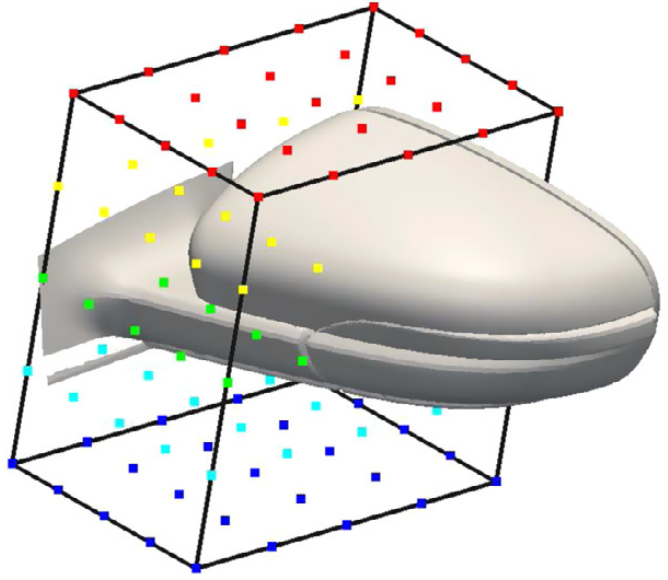
\includegraphics[width=0.7\textwidth]{./img/ridici_body.png}
	\caption{Řídící body objemového B-spline okolo automobilového zrcátka. Příklad z \cite{papoutsis2015noise}.}
	\label{fig:zrcatko}
\end{figure}


\section{Optimalizacni cyklus}

flowchart s naznacenim kde kdy se jake rovnice pocitaji (hlavni NS-rce, sdruzene rce, pohyb site)

\begin{figure}
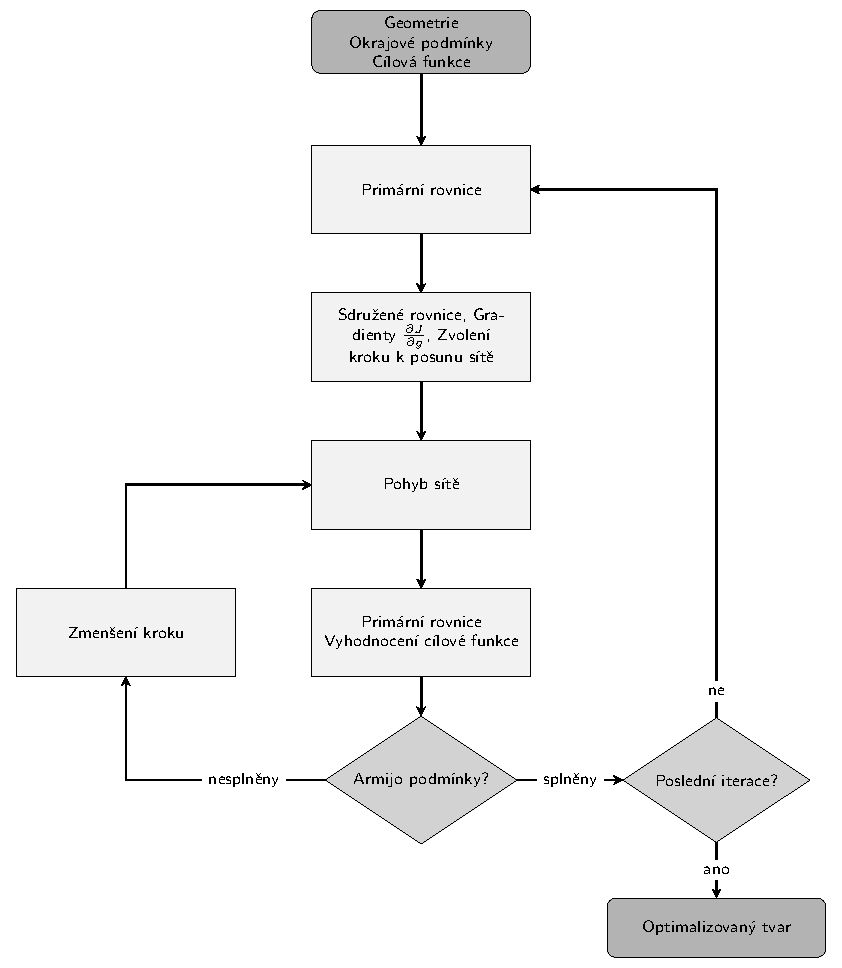
\includegraphics[width=0.9\textwidth]{./img/flowchart/optimalizacni_cyklus.pdf}
\caption{Optimalizacni cyklus}
\label{fig:flowchart_opt_cyklus}
\end{figure}









\part{Praktická aplikace}
%!TEX ROOT=../_main.tex

\chapter{Tvarová optimalizace kompresorové mříže}

Tato kapitola prezentuje použitou metodiku pro optimalizaci tvaru lopatky v kompresorové mříži pomocí sdružené metody a knihovny OpenFOAM pro simulace metodou konečných objemů.

\section{Obecný popis problému}

Simulace prováděné v rámci této práce zjednodušeně reprezentují měřící soustavu tzv. lopatkových mříží. Pro lopatkové mříže jsou určující zejména geometrie samotné lopatky, rozteč $ t $ jednotlivých lopatek a stav proudu před a za mříží.

V rámci numerické simulace je topologie výpočetní oblasti naznačena na obrázku \ref{fig:vypocetni_oblast}. Vstupní a výstupní hranice jsou rovnoběžné s osou y a jejich výška je právě zmiňovaný parametr rozteče $ t $. Uprostřed oblasti se nachází uzavřená hranice reprezentující geometrii lopatky. Vrchní a spodní hranice jsou brány jako periodické, tedy to co vyteče spodem, vteče vrchem a naopak. Prostorová diskretizace (síť) je v této práci vždy dělána tak, aby si stěny buněk na obou stranách periodické hranice odpovídali $ 1:1 $, pouze s posunutím $ t $.

\begin{figure}
	\def\svgwidth{0.8\textwidth}
	\graphicspath{{img/inkscape/}}
	\includesvg{img/inkscape/comp_domain}
%	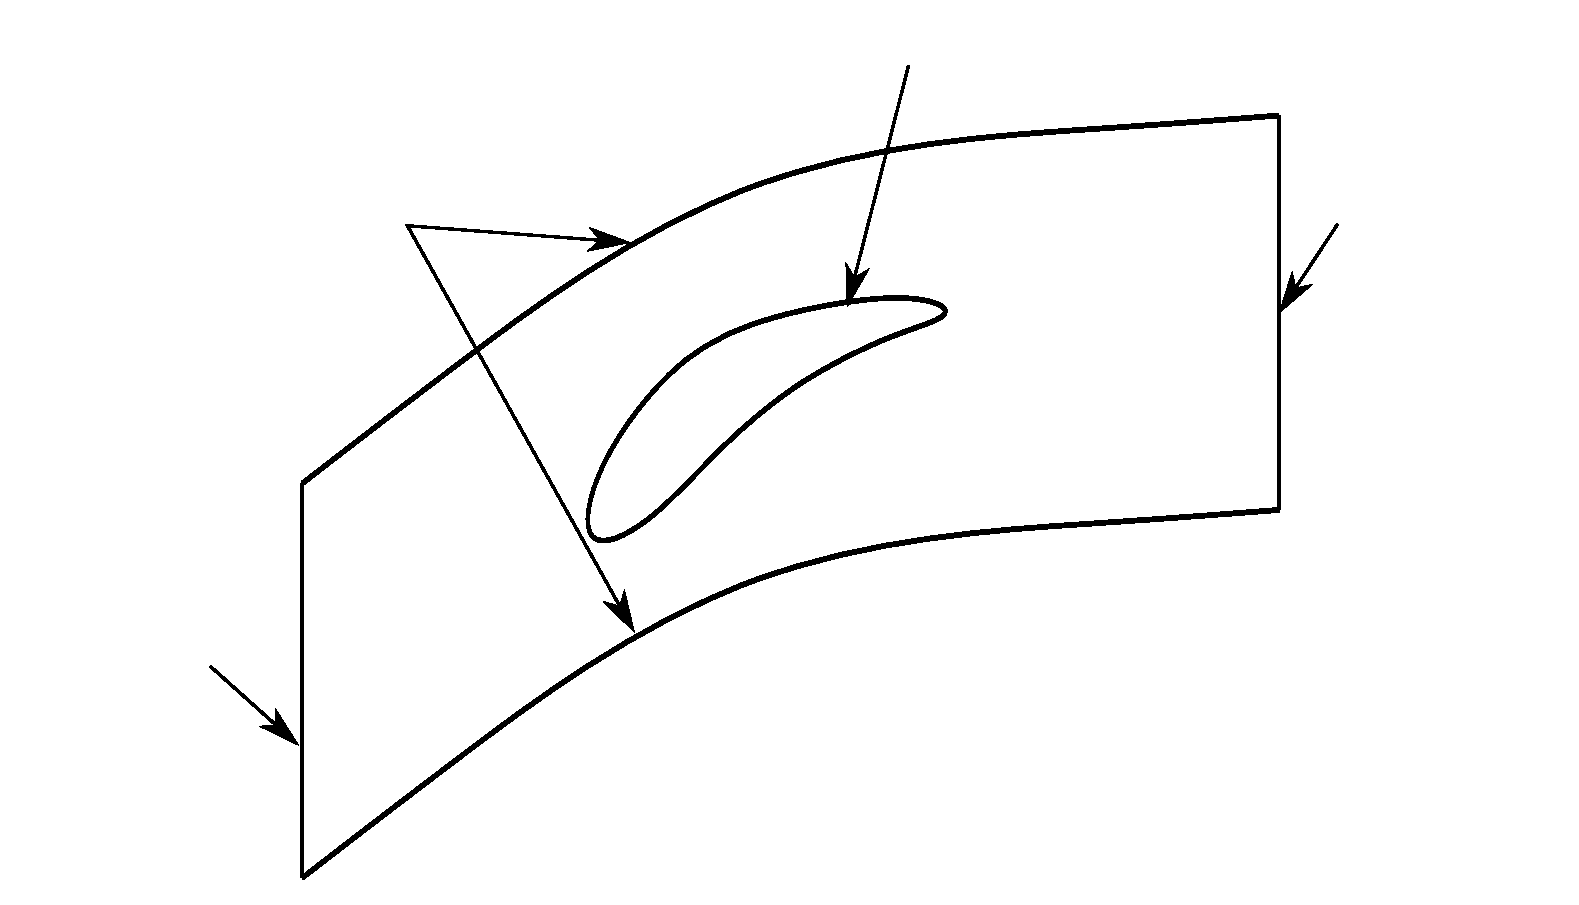
\includegraphics[width=0.7\textwidth]{img/inkscape/comp_domain.pdf}
	\caption[Topologie výpočetní oblasti]{Náčrt topologie výpočetní oblasti pro standardní axiální kompresorovou mříž.}
	\label{fig:vypocetni_oblast}
\end{figure}

Krom periodicity jsou další okrajové podmínky následující. Na vstupu je předepsána Dirichletova okrajová podmínka pro vektor rychlosti a turbulentní proměnné. Tlak zde má nulovou Neumanovu podmínku. Na výstupu je naopak statický tlak fixován na nulu a rychlost je zde předepsána pomocí nulového gradientu.

\section{Cílové funkce}

V rámci aplikace sdružené optimalizace na tvar lopatky kompresorové mříže lze vymyslet hned několik cílů. V jednom stupni axiálního kompresoru se běžně sledují veličiny stlačení, účinnost (respektive ztráty) a výstupní úhel proudu. Pro tuto práci se jako sledovaná a optimalizovaná veličina bere ta poslední, tedy výstupní úhel proudu $ \alpha_2 $. 

K dosažení cílového úhlu na výstupu z lopatkové mříže $ \alpha_{2tar} $ jsou použity dva postupy. Oba vycházejí z definice úhlu výstupního proudu
\begin{equation}\label{eq:alpha_tan}
\alpha_2 = \arctan\left(\dfrac{u_{y2}}{u_{x2}}\right).
\end{equation}
Ze zákona zachování hmotnosti pro proudění nestlačitelné tekutiny vyplývá, že to co do kontrolní oblasti vteče, musí i vytéct. Jinými slovy toky vstupní a výstupní hranicí se musejí rovnat
\begin{equation}
\dot{m_1}=\dot{m_2},
\end{equation}
což pro proudění nestlačitelné tekutiny kontrolní oblastí s vstupní a výstupní hranicí rovnoběžnou s osou y znamená, že 
\begin{equation}\label{eq:ux1_ux2}
u_{x1}=u_{x2}.
\end{equation}
Okrajové podmínky definují na vstupu konstantní uniformní vektor rychlosti $ \mathbf{u_1} $ a přeneseně tedy i x-ovou složku rychlosti na výstupu. Z toho vyplývá, že pro zadané $ \alpha_{2tar} $ můžeme apriori spočítat
\begin{equation}
u_{y2tar} = \tan(\alpha_{2tar}) \cdot u_{x2},
\end{equation}
tedy jistou cílovou rychlost na výstupu a cílovou funkci formulovat pomocí ní.

Dále jsou srovnány dvě formulace cílové funkce. První formulace optimalizuje přímo výstupní složku rychlosti, kdežto druhá optimalizuje nepřímo přes sílu na lopatku.

Zatímco přímá formulace ovlivňuje přes derivaci cílové funkce okrajovou podmínku sdružených rovnic pouze na výstupní hranici $ \Gamma_2 $, cílová funkce přes sílu ovlivňuje okrajovou podmínku na lopatce $ \Gamma_P $. Druhým rozdílem je pak, že v přímé formulaci se objevuje jediná primární proměnná, kdežto pro integraci síly na lopatce jsou potřeba všechny proměnné, včetně turbulentní proměnné $ \widetilde{\nu} $. Tyto rozdíly zavdávají dostatečný důvod pro zkoumání a porovnání těchto dvou formulací ve smyslu rychlosti konvergence a přesnosti.

\subsection{Přímá formulace}

V přímé formulaci se snažíme aby
\begin{equation}
	u_{y2tar}=\dfrac{1}{\phi_2}\sum_{f\in\Gamma_2}\phi_f u_{yf},
\end{equation}
tedy aby průměr $ u_y $ na výstupu vážený přes hmotnostní tok byl roven zadané cílové rychlosti.
Minimalizovanou cílovou funkci formulujeme jako
\begin{equation}\label{eq:J_UyTarget}
	J = \int_{\Gamma_2}\left( u_y(y)-u_{y2tar} \right)^2\mathrm{d}S = \int_{\Gamma_2} J_\Gamma\, \mathrm{d}S.
\end{equation}
Ve smyslu vztahu \ref{eq:cenova_fce} má takto definovaná cílová funkce pouze hraniční složku $ J_\Gamma $ a pro sdružené rovnice tak bude figurovat pouze v hraničních členech, tedy v rovnicích \ref{eq:sdruzenaOP1} a \ref{eq:sdruzenaOP2}. Potřebujeme tedy vydefinovat parciální derivace podle primárních proměnných $ \mathbf{u} $ a $ p $. Pro implementaci v rámci knihovny OpenFOAM je pak navíc potřeba vydefinovat ještě derivace podle $ u_n $ a $ u_t $, což pro dříve definovanou úlohu znamená podle složek $ u_x $ a $ u_y $.

Parciální derivace podle primárního tlaku $ \dfrac{\partial}{\partial p} $ je nulová, neboť tlak v cílové funkci nefiguruje.

Pro parciální derivaci podle primární rychlosti $ \mathbf{u} $ je lepší se dívat na složku $ u_y $ jako na skalární součin $ \mathbf{u}\cdot \mathbf{j}=\mathbf{u}\cdot (0,1,0) = u_y$ a derivaci tedy provést jako
\begin{equation}\label{key}
\dfrac{\partial J_\Gamma}{\partial \mathbf{u}}
=
\dfrac{\partial \left( \mathbf{u}\cdot \mathbf{j}-u_{y2tar} \right)^2}{\partial \mathbf{u}}
=
2( \mathbf{u}\cdot \mathbf{j}-u_{y2tar} )\,\mathbf{j}
=
2( u_y-u_{y2tar} )\,\mathbf{j}.
\end{equation}
U dodatečných derivací pro OpenFOAM vychází $ \dfrac{\partial}{\partial u_n}=0 $ a $ \dfrac{\partial }{\partial u_t} $ je stejná jako derivace podle $ \mathbf{u} $.

\subsection{Nepřímá formulace přes sílu}

Druhou možností jak dosáhnout zadaného úhlu výstupního proudu je použít optimalizaci přes cílovou sílu. 
Optimalizace síly na stěnu ve smyslu její minimalizace v předepsaném směru je v balíku OpenFOAM formulována jako
\begin{equation}\label{eq:J_FyOForig}
J_{OF}=\dfrac{\int_\Gamma \rho (-\tau_{ij}n_j+pn_i)r_i\,\mathrm{d}S}{\frac{1}{2}\rho A U_{\infty}^2},
\end{equation}
kde $ \tau_{ij} $ jsou složky tenzoru napětí, $ p $ tlak dělený konstantní hustotou $ \rho $ a $ \mathbf{n} $ jednotkový normálový vektor. Vektor $ \mathbf{r} $ pak definuje směr projekce vektoru síly (směr ve kterém se minimalizuje). $ A $ je referenční plocha a $ U_{\infty} $ je rychlost volného proudu. Takto definovaná cílová funkce tedy svou velikostí odpovídá koeficientu síly $ C_f $.

Pro potřeby optimalizace na cílovou sílu $ F_{yPtar} $ bylo vhodnější použít přímo samotnou sílu, tedy pouze čitatel v rovnici \ref{eq:J_FyOForig}, a za vektor projekce brát jednotkový vektor ve směru osy y. Pro celkovou sílu působící na lopatku ve směru y tak lze psát
\begin{equation}\label{key}
F_{yP}=\int_{\Gamma_P} \rho (-\tau_{ij}n_j+pn_i)\delta_{i2}\,\mathrm{d}S.
\end{equation}
Absolutní velikost takto vyhodnocené síly samozřejmě závisí i na rozměru lopatky v ose z. Číselné výsledky uváděné později jsou uváděny vždy relativní, takže nezávisí na libovolné konstantní výšce lopatky. Cílovou funkci pro cílovou sílu tak definujeme podobně jako pro rychlost přes kvadrát rozdílu, tedy
\begin{equation}\label{eq:J_FyTarget}
J= (F_{yP} - F_{yPtar})^2.
\end{equation}
Pro derivaci této cílové funkce podle libovolné proměnné $ w $ pak platí
\begin{equation}\label{key}
\dfrac{\partial J}{\partial w} = 
2(F_{yP}-F_{yPtar}) \cdot \dfrac{\partial F_{yP}}{\partial w}.
\end{equation}
Výraz $ \frac{\partial F_{yP}}{\partial w} $ odpovídá derivaci čitatele (anglicky \textit{nominator}, $ \mathrm{nom()} $) cílové funkce definované rovnicí \ref{eq:J_FyOForig}, tedy
\begin{equation}\label{key}
\dfrac{\partial F_{yP}}{\partial w} = \dfrac{\partial (\mathrm{nom}(J_{OF}))}{\partial w}.
\end{equation}
Pro tuto cílovou funkci tedy nebylo potřeba odvozovat potřebné derivace a stačilo pouze vynásobit příslušné výrazy definované v kódu knihovny OpenFOAM výrazem $ 2(F_{yP}-F_{yPtar}) $.



\section{Optimalizace mříže GHH 1-S1}
Pro aplikaci nově zpracovaných cílových funkcí byla zvolena axiální kompresorová mříž MAN GHH 1-S1 publikovaná v \cite{steinert1990design}.
Výpočetní oblast topologicky odpovídá náčrtu na obrázku \ref{fig:vypocetni_oblast}.
Rozteč lopatek v mříži je $ t=0.0476\,\mathrm{m} $. Hustota tekutiny používaná při vyhodnocení síly je $ \rho=1.225\,\mathrm{kg\,m^{-3}} $ a kinematická viskozita $ \nu = 1.5\cdot10^{-5} \, \mathrm{m^2s^{-1}} $.

\subsection{Okrajové podmínky}  Na vstupu je Machovo číslo $ M=0.62 $ a úhel proudu $ \alpha_1 = 47^\circ $, což při klidové rychlosti vzduchu $ c=340 \,\mathrm{m\,s^{-1}} $ vede na okrajovou podmínku pro vstupní rychlost  
\begin{equation}\label{key}
\mathbf{u_1}=M\cdot c \cdot (\cos(\alpha_1),\, \sin(\alpha_1),\, 0) \doteq (143.8,\, 154.2,\, 0)\, \mathrm{m\,s^{-1}}.
\end{equation}
Kinematický tlak na výstupu je fixován $ p_2=0\,\mathrm{m^2s^{-2}} $.

\subsection{Modelování turbulence}
Modelování turbulence se realizuje pomocí přídavné turbulentní vazkosti. Pro zjištění turbulentní vazkosti $ \nu_t $ je v optimalizačním algoritmu použit model Spalart-Allmaras\cite{spalart1992one}. Jelikož ale tento model je původně navržen pro obtékání profilu křídla ve volném proudu, není ve své původní variantě vhodný pro modelování turbulence ve vnitřní aerodynamice, kam kompresorové mříže spadají. Knihovna OpenFOAM prozatím ale neobsahuje sdružené rovnice pro žádný jiný model turbulence než Spalart-Alamaras a odvození sdružených rovnic pro pokročilejší model turbulence je nad rámec této práce, byl použit následující postup. 

Ve výchozí konfiguraci byla provedena simulace s vhodnějším modelem $k\text{-}\omega$ SST implementovaným v knihovně OpenFOAM na základě \cite{menter1994two, menter2003ten, rumsey2013menter} s následujícími okrajovými podmínkami na vstupu. Intenzita turbulence na vstupu $ I=2\% $, tedy odkud plyne Dirichletova podmínka pro turbulentní kinetickou energii $ k $ ze vztahu  \begin{equation}\label{key}
k=1.5(I|\mathbf{u}|)^2.
\end{equation} 
Turbulentní směšovací délka $ L_t=0.002\,\mathrm{m} $, odkud plyne Dirichletova okrajová podmínka pro $ \omega $ ze vztahu
\begin{equation}\label{key}
\omega=\dfrac{k^{0.5}}{C_\mu^{0.25}L_t};\,\, C_\mu=0.09\,.
\end{equation} 
Ve výchozí konfiguraci bylo následně provedeno několik simulací s modelem Spalart-Allmaras, kde se variovala vstupní hodnota turbulentní proměnné tohoto modelu $ \tilde{\nu}_1 $ z intervalu $ \langle 10^{-6},10 \rangle $. Pro každý výpočet byl vyhodnocen koeficient ztráty celkového tlaku podle vztahu z \cite{steinert1990design}
\begin{equation}\label{key}
\omega = \dfrac{p_{t1}-p_{t2}}{p_{t1}-p_1}
\end{equation}
a poměr celkových tlaků $ \frac{p_{t1}}{p_{t2}} $. Pro další simulace této lopatkové mříže pak byla na vstupu zvolena Dirichletova podmínka $ \tilde{\nu} = 3.4\cdot 10^{-4} $ neboť pro tuto hodnotu vyšel relativní rozdíl v předpovědi modelem Spalart-Allmaras oproti $k\text{-}\omega$ SST pro obě vyhodnocované veličiny pod $ 1\% $.

\subsection{Prostorová diskretizace}

Výpočetní oblast byla diskretizována na množinu vzájemně disjunktních objemů. Dvourozměrná síť byla vytvořena v softwaru ANSYS ICEM a její detail je ukázán na obrázku \ref{fig:ghs1_sit}. Následný převod sítě do formátu pro OpenFOAM (2D síť na pseudo-3D) byl proveden s parametrem 0.01 pro souřadnice $ z $.

\begin{figure}
	\centering
	\def\svgwidth{1\textwidth}
	\graphicspath{{img/inkscape/}}
	\includesvg{img/inkscape/wireframe}
	\caption[Výpočetní síť mříže GHH 1-S1]{Výpočetní síť pro lopatkovou mříž GHH 1-S1 s detailem náběžné a odtokové hrany. Síť sestává z celkem 85 tisíc hexahedrálních buněk. }
	\label{fig:ghs1_sit}
\end{figure}

Síť byla tvořena s důrazem na co nejlepší zachycení mezní vrstvy. Buňky v oblasti okolo lopatky jsou exponenciálně zmenšovány, aby se dosáhlo $ y^+ < 1 $ a nebylo tak nutné používat stěnové funkce ani pro jeden z turbulentních modelů.
S touto sítí ve výchozí konfiguraci s modelem $k\text{-}\omega$ SST je dosaženo $ \max\limits_{\Gamma_P}(y^+) \doteq 0.39 $. Validita této sítě byla ověřena metodou \textit{Grid convergence index} (zkráceně GCI) v \cite{tater2021mesh}.


\subsubsection{Řídící body objemových B-spline}
Pro transformaci tvaru lopatky a pohybu se sítí pomocí objemových B-spline je potřeba vydefinovat řídící body. Z experimentů s různým rozdělením řídících bodů a jejich fixací v průběhu optimalizačních cyklů vzešlo, že stabilita řešení sdružených rovnic i konečný výsledek optimalizace na rozdělení řídících bodů závisí víc než by se dalo označit za uživatelsky příjemné. Konečné rozdělení řídících bodu je ukázáno na \ref{fig:ghs1_cps}. Ve směru $ u $, který koresponduje se směrem osy $ x $, bylo zvoleno 14 vrstev bodů a ve směru $ v $ pak 6. Fixované v průběhu simulace byly všechny krajní body. Druhá a předposlední vrstva ve směru $ u $ (sloupec) má pak zakázán pohyb ve směru osy $ x $. Vrstvy ve směru $ u $ procházející náběžnou a odtokovou hranou profilu mají zakázán pohyb úplně. Cílem těchto omezení je fixovat pozici začátku a konce lopatky, aby nedošlo k natahování lopatky a deformaci odtokové hrany. Tento nechtěný efekt měl tendenci nastat pokud se fixovaly například pouze vnější body.

\begin{figure}
	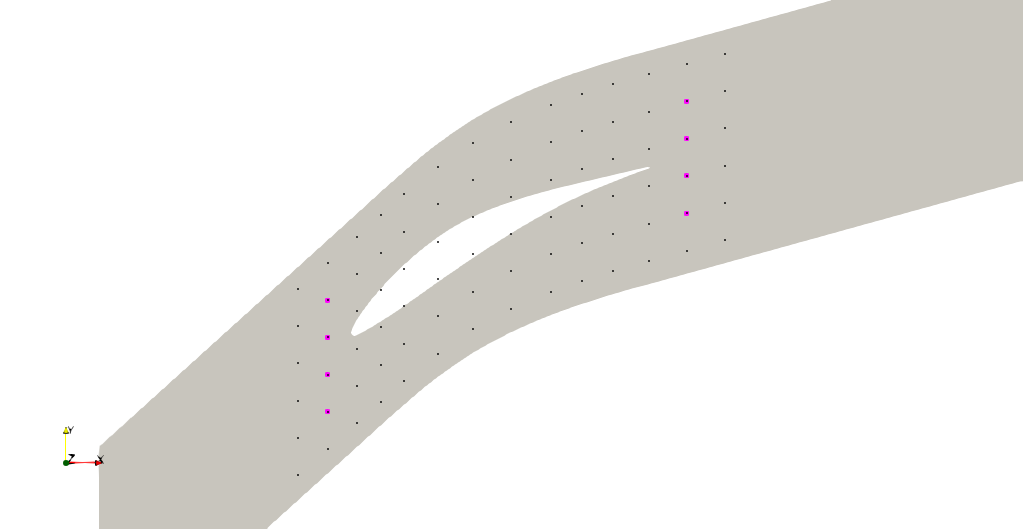
\includegraphics[width=0.75\textwidth]{img/cps.png}
	\caption[Pozice řídících bodů]{Pozice řídících bodů objemových B-spline ve výpočetní oblasti pro lopatkovou mříž GHH 1-S1. Růžové body se smí pohybovat pouze ve směru osy $ y $.}
	\label{fig:ghs1_cps}
\end{figure}


\subsection{Parametry optimalizace}
Cílové funkce používané pro optimalizaci jsou definovány rovnicemi \ref{eq:J_UyTarget} a \ref{eq:J_FyTarget}, tedy optimalizace přímá na $ u_{y2tar} $ a nepřímá na $ F_{yPtar} $. Optimalizace tvaru lopatky byla dodatečně omezena, tak aby průřez lopatky zůstal konstantní, což lze pro trojrozměrný prostor matematicky formulovat jako
\begin{equation} 
V=-1/3\int_{\Gamma_P}x_kn_k\mathrm{d}S.
\end{equation}

Kvůli přidané podmínce konstantního průřezu byla jako metoda aktualizace zvolena metoda projekce omezení (anglicky \textit{constraint projection}). Výchozí krok ve směru gradientu $ \eta $ je v první iteraci spočítán podle maximálního povoleného pohybu sítě, který byl nastaven na $ 5\cdot10^{-4} $. Velikost kroku $ \eta $ se posléze v jednotlivých iteracích zmenšuje podle Armijo podmínky jak definuje \cite{nocedal1999numerical}. Tento cyklus zmenšuje krok $ \eta^{k+1}=0.75\cdot\eta^{k} $ a vyhodnocuje hodnotu cílové funkce $ J $ (tedy simuluje primární rovnice), než jsou splněny dané podmínky. Pro Armijo podmínky je důležitý koeficient $ c1 $, který byl zvolen $ 10^{-3} $.

Výstupní úhel proudu byl ve výchozí konfiguraci s modelem Spalart-Allmaras $ \alpha_{2}^{0}=21.46^{\circ} $. Cílové výstupní úhly byly zvoleny z množiny $ \langle \alpha_{2}^{0}-4^{\circ}, \alpha_{2}^{0}+8^{\circ} \rangle $ s krokem $ 2^{\circ} $. Celkem tedy 6 různých cílových úhlů.

\subsection{Výsledky optimalizace} \label{sec:vysledky_opt}
K dosažení cílového úhlu výstupního proudu byla použita nejdříve přímá formulace cílové funkce. Následně, když optimalizace bylo nalezeno optimální řešení, byla vyhodnocena síla $ F_{yP} $ působící na lopatku. Tato síla pak byla použita jako cílová síla $ F_{yPtar} $ pro nepřímou formulaci cílové funkce. Konkrétní cílové hodnoty s odpovídajícími cílovými úhly jsou uvedeny v tabulce \ref{tab:cilove_hodnoty}.

\begin{table}
	\begin{ctucolortab}
		\begin{tabular}{c|c||c|c}
			
			$ \Delta\alpha_{2} $ &$ \alpha_{2tar} $ & $ u_{y2tar}\,[\mathrm{ms^{-1}}] $ & $ F_{yPtar}\,[\mathrm{N}] $ \\
			\hline
			-4° & 17.46° & 45.32 & 9.12 \\
			
			-2° & 19.46° & 50.91 & 8.65 \\
			
			+2° & 23.46° & 62.53 & 7.69 \\
			
			+4° & 25.46° & 68.60 & 7.17 \\
			
			+6° & 27.46° & 74.87 & 6.65 \\
			
			+8° & 29.46° & 81.38 & 6.10 \\
			
		\end{tabular}
	\end{ctucolortab}
	\caption{Cílové hodnoty pro optimalizaci.}
	\label{tab:cilove_hodnoty}
\end{table}

\subsubsection{Optimalizace $ u_{y2} $}


Pro vyhodnocení konvergence optimalizace s přímou formulací cílové funkce je jako určující norma (residuum) pro každou iteraci $ i $ brán relativní rozdíl
\begin{equation}\label{eq:res_uy}
Res_{u_{y}}^i=\dfrac{|u_{y2}^i-u_{y2tar}|}{|u_{y2}^0|}.
\end{equation}
Residua pro všechny cílové hodnoty v průběhu optimalizačních cyklů jsou ukázány na obrázku \ref{fig:ghs1_Uy}.
Optimalizaci pak považujeme za zkonvergovanou, pokud residuum klesne pod jedno procento. Na obrázku \ref{fig:ghs1_Uy} je hranice konvergence naznačena růžovou čarou.

Jelikož ale ve výsledku chceme optimalizovat hodnotu výstupního úhlu, je rozumné se dívat i na residuum vzhledem k $ \alpha_2 $, tedy na 
\begin{equation}\label{eq:res_alpha}
Res_{\alpha}^i=\dfrac{|\alpha_{2}^i-\alpha_{2tar}|}{|\alpha_{2}^0|}.
\end{equation}
Graf residuí $ Res_{\alpha}^i $ na obrázku \ref{fig:ghs1_UyA} je samozřejmě pro přímou formulaci velice podobný grafu residua samotné optimalizace, neboť $ \alpha_2 $ se z $ u_{y2} $ přímo vyhodnocuje podle vztahu \ref{eq:alpha_tan}. Teoreticky by měly být grafy naprosto stejné, neboť $ u_{x2} $ by mělo být podle vztahu \ref{eq:ux1_ux2} pro všechny případy stejné. Vlivem chyb diskretizace tomu tak úplně není a grafy se tak pro malé hodnoty residua drobně liší.

Dále lze z grafu residuí vypozorovat, že čím větší je rozdíl $ \Delta \alpha_{2} = \alpha_{2tar} - \alpha_{2}^{0}$, tím déle trvá optimalizaci zkonvergovat. To samozřejmě odpovídá očekávání. Při porovnání rychlosti konvergence optimalizace do záporných versus do kladných úhlu výstupního proudu lze říci, že optimalizovat do kladných úhlů je pro takto nastavený optimalizační algoritmus jednodušší. Optimalizace do kladných úhlů odpovídá napřimování tvaru lopatky, kdežto při optimalizaci do záporných úhlů je pro dosažení cílové hodnoty úhlu výstupního proudu potřeba lopatku ohnout více. Tento zmiňovaný rozdíl lze nejlépe vidět při porovnání případů $ \alpha_{2tar}=\pm 4^{\circ} $. Pro kladný úhel +4° je optimální řešení nalezeno už v 9. iteraci, kdežto při ohýbání lopatky k dosažení záporného $ \Delta\alpha $ je potřeba optimalizačních cyklů 12.

\begin{figure}[H]
	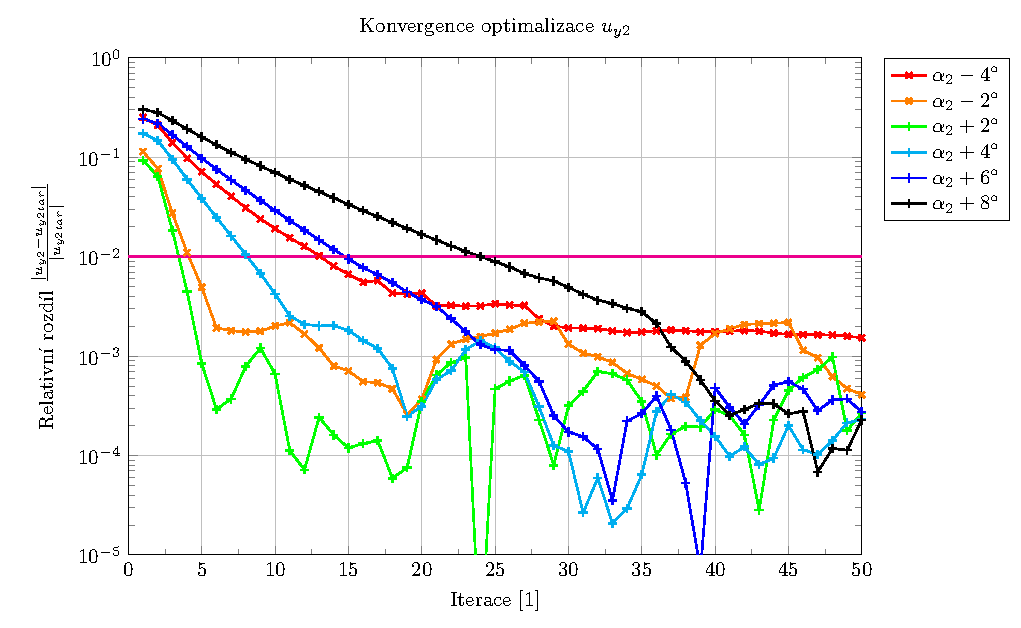
\includegraphics[width=0.95\textwidth]{img/Uy.pdf}
	\caption[Průběh residua $ Res_{u_y}^i $]{Průběh residua $ Res_{u_y}^i $ \ref{eq:res_uy} pro přímou formulaci cílové funkce $ J $ v průběhu iteračních cyklů. Hranice optimálního řešení $ 1\% $ je naznačena růžovou čarou.}
	\label{fig:ghs1_Uy}
\end{figure}

\begin{figure}[H]
	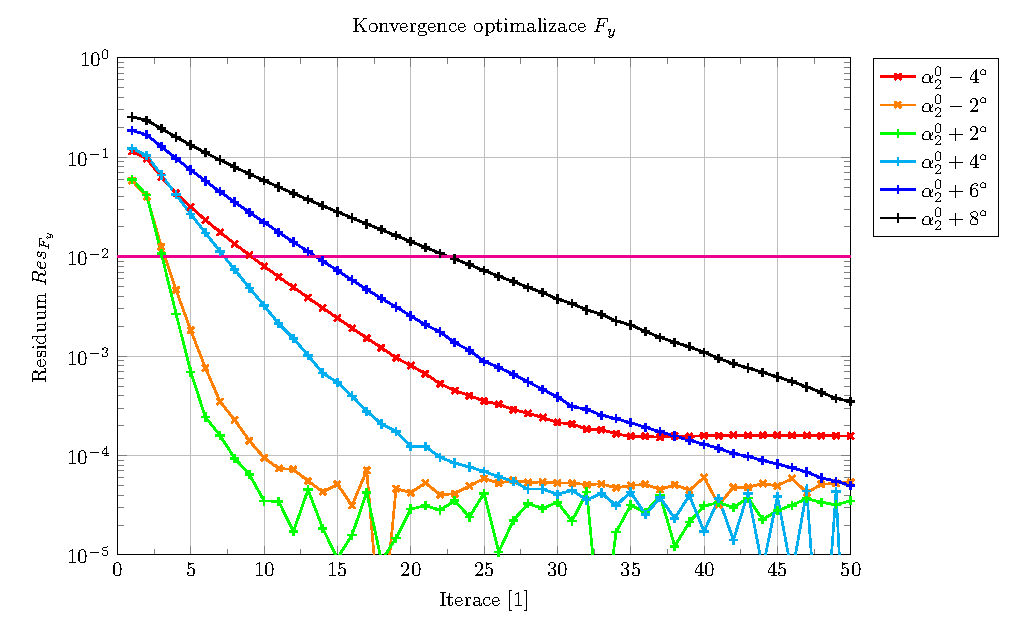
\includegraphics[width=0.95\textwidth]{img/Fy.pdf}
	\caption[Průběh residua $ Res_{F_y}^i $]{Průběh residua $ Res_{F_y}^i $ \ref{eq:res_fy} pro nepřímou formulaci cílové funkce $ J $ v průběhu iteračních cyklů. Hranice optimálního řešení $ 1\% $ je naznačena růžovou čarou.}
	\label{fig:ghs1_Fy}
\end{figure}

\subsubsection{Optimalizace $ F_{yP} $}

Pro vyhodnocení optimálnosti řešení pro nepřímou formulací cílové funkce je jako residuum pro každou iteraci $ i $ brán relativní rozdíl
\begin{equation}\label{eq:res_fy}
Res_{F_{y}}^i=\dfrac{|F_{yP}^i-F_{yPtar}|}{|F_{yP}^0|}.
\end{equation}
Stejně jako pro přímou formulaci bereme hranici optimálního řešení jedno procento. Residua pro všechny cílové hodnoty v průběhu optimalizačních cyklů pro nepřímou formulaci cílové funkce jsou ukázány na obrázku \ref{fig:ghs1_Fy} s naznačenou hranicí konvergence. 

V porovnání s grafem konvergence \ref{fig:ghs1_Uy} pro přímou formulaci cílové funkce průběh residua \ref{fig:ghs1_Fy} o poznání méně osciluje. To si lze vysvětlit tím, že pro vyhodnocení cílové funkce pro sílu (a jejích derivací) jsou použity všechny primární proměnné a tedy se využívá více informací z proudového pole pro předpověď gradientu. Na základě tohoto pozorování lze s opatrností usoudit, že optimalizace na cílovou sílu je značně stabilnější než optimalizace na cílovou výstupní rychlost. Zároveň optimalizační algoritmus zkonverguje v méně iteracích než tomu bylo pro přímou formulaci cílové funkce. Například pro případ $ \Delta \alpha = +8^\circ $ stačilo o pět iterací méně. V tomto smyslu by bylo zajímavé i porovnání průběhu residuí jako funkce výpočetního času. V současné konfiguraci optimalizačních algoritmů byl celkový čas výpočtu (pro 50 iterací) vždy nižší pro přímou formulaci. Ve zmiňovaném případě $ \Delta \alpha = +8^\circ $ byl celkový výpočetní čas pro přímou formulaci $ 2265 \,\mathrm{s} $ a pro nepřímou formulaci $ 2927 \,\mathrm{s} $.

\begin{figure}[H]
	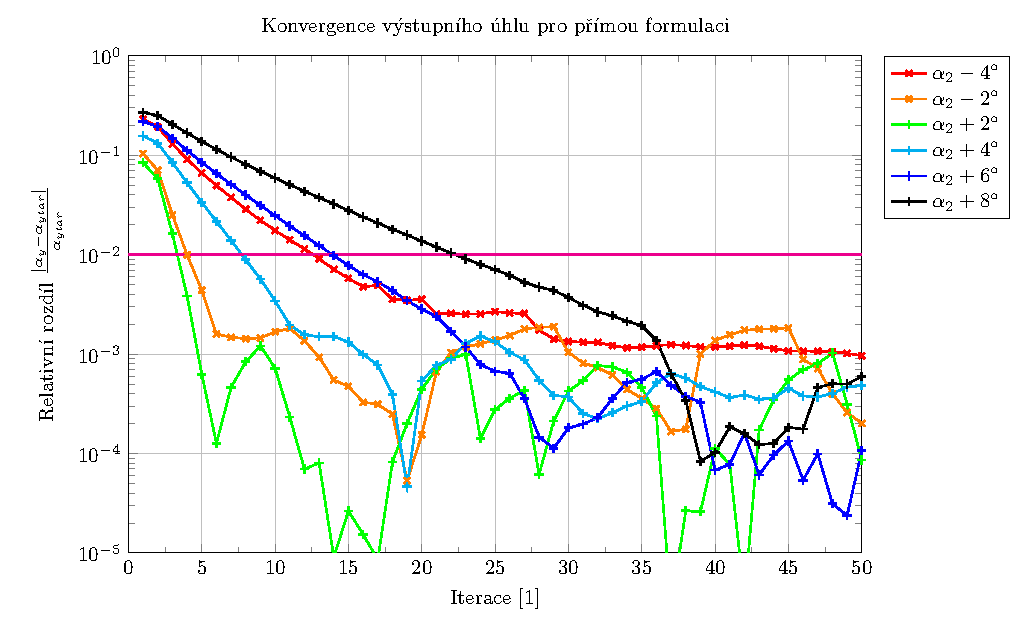
\includegraphics[width=0.9\textwidth]{img/UyA.pdf}
	\caption[Průběh residua $ Res_{\alpha}^i $, přímá formulace]{Průběh residua $ Res_{\alpha}^i $ \ref{eq:res_alpha} pro přímou formulaci cílové funkce $ J $ v průběhu iteračních cyklů. Hranice optimálního řešení $ 1\% $ je naznačena růžovou čarou.}
	\label{fig:ghs1_UyA}
\end{figure}

\begin{figure}[H]
	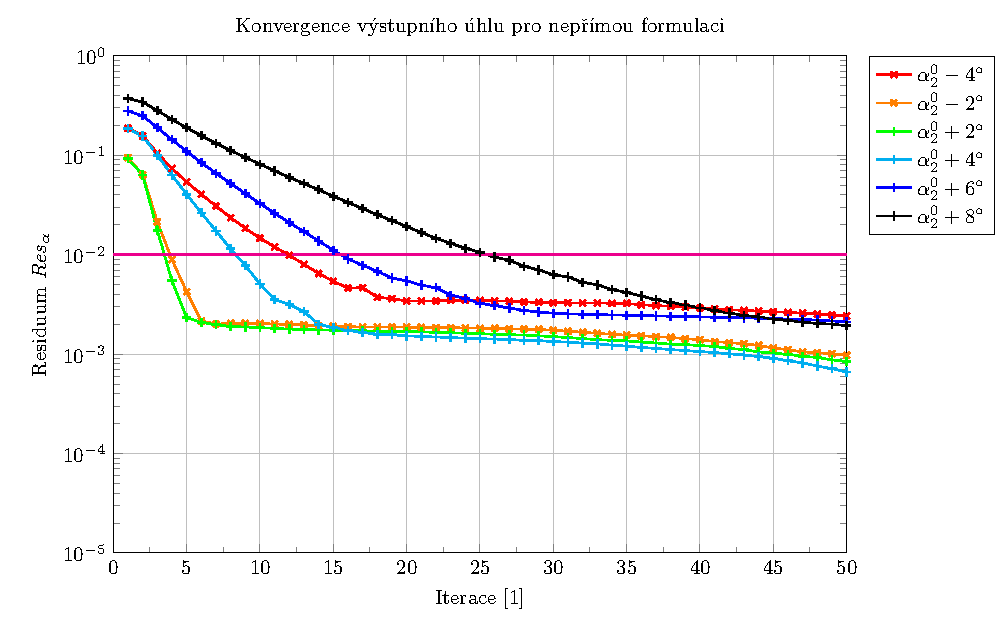
\includegraphics[width=0.9\textwidth]{img/FyA.pdf}
	\caption[Průběh residua $ Res_{\alpha}^i $, nepřímá formulace]{Průběh residua $ Res_{\alpha}^i $ \ref{eq:res_alpha} pro nepřímou formulaci cílové funkce $ J $ v průběhu iteračních cyklů. Hranice optimálního řešení $ 1\% $ je naznačena růžovou čarou.}
	\label{fig:ghs1_FyA}
\end{figure}

Optimalizaci na cílovou sílu používáme k nepřímému dosažení žádaného výstupního úhlu proudu. Proto je důležitější podívat se na graf konvergence ve smyslu vztahu \ref{eq:res_alpha}, který je na obrázku \ref{fig:ghs1_FyA}. Nejmarkantnějším rozdílem v porovnání s grafem \ref{fig:ghs1_UyA} je průběh residua pod hranicí konvergence, který je opět hladší. Nejdůležitější srovnání je ale v počtu iterací potřebných ke zkonvergování $ \alpha_2 $. Na rozdíl od porovnání cílových residuí $ Res_{u_y}^i $ a $ Res_{F_y}^i $ je počet potřebných iterací pro všechny případy $ \Delta\alpha_2 $ stejný. Jak bylo ale zmíněno v předchozím odstavci, optimalizace s přímou formulací cílové funkce je ve všech případech rychlejší. Na základě tohoto porovnání lze bezpečně říci, že pro případ optimalizace lopatky GHH 1-S1 na takto kvalitní síti nepřináší nepřímá formulace žádné benefity. Pro jiné případy tomu tak ovšem být nemusí, neb z průběhu cílových residuí \ref{eq:res_uy} a \ref{eq:res_fy} lze usoudit, že optimalizace na cílovou sílu je mnohem stabilnější, což může hrát ve složitějších aplikacích důležitou roli.
\newpage
\subsubsection{Srovnání pro $ \Delta \alpha_2=-4^{\circ} $}

Porovnání tvaru lopatky je provedeno mezi původním tvarem profilu a profilem z optimalizace zkorvergované ve smyslu $ Res_{\alpha}^i $. Pro $ \alpha_2=-4^\circ $ to je profil ze 12. iterace optimalizačního algoritmu.

\begin{figure}[H]
	\centering
	\def\svgwidth{0.8\textwidth}
	\graphicspath{{img/inkscape/}}
	\includesvg{img/inkscape/prof_wire}
	\caption[Tvar optimalizované lopatky]{Obrys tvaru lopatky před optimalizací (černě) a po optimalizaci s přímou (modře) a nepřímou (červeně) formulací cílové funkce. Červená křivka na většině obrázku překrývá modrou.}
	\label{fig:ghs1_alphaminus4}
\end{figure}

\begin{figure}[H]
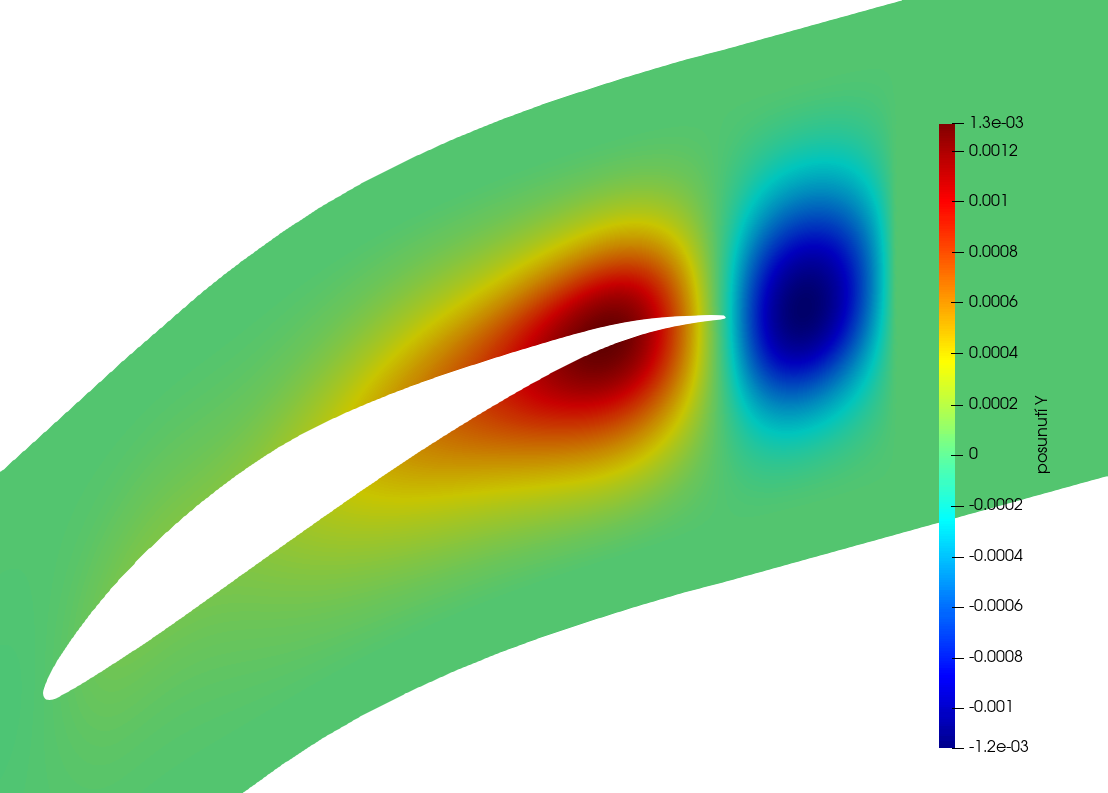
\includegraphics[width=0.75\textwidth]{img/displacement_12.png}
\caption[Pole posunutí sítě]{Vizualizace pole posunu bodů sítě ve směru osy $ y $.}
\label{fig:ghs1_disp12}
\end{figure}

Zajímavé je srovnání optimalizovaných tvarů lopatky získaných přímou a nepřímou formulací. Jak je vidět na obrázku \ref{fig:ghs1_alphaminus4}, tvar optimalizovaných profilu je v podstatě totožný. Obě formulace pohybují především s částí lopatky v blízkosti odtokové hrany jak je vidět z obrázku \ref{fig:ghs1_disp12}. To dává smysl, neboť koncová část lopatky má často mnohem větší vliv na směr proudu na výstupu než část u náběžné hrany.
\begin{figure}[h]
	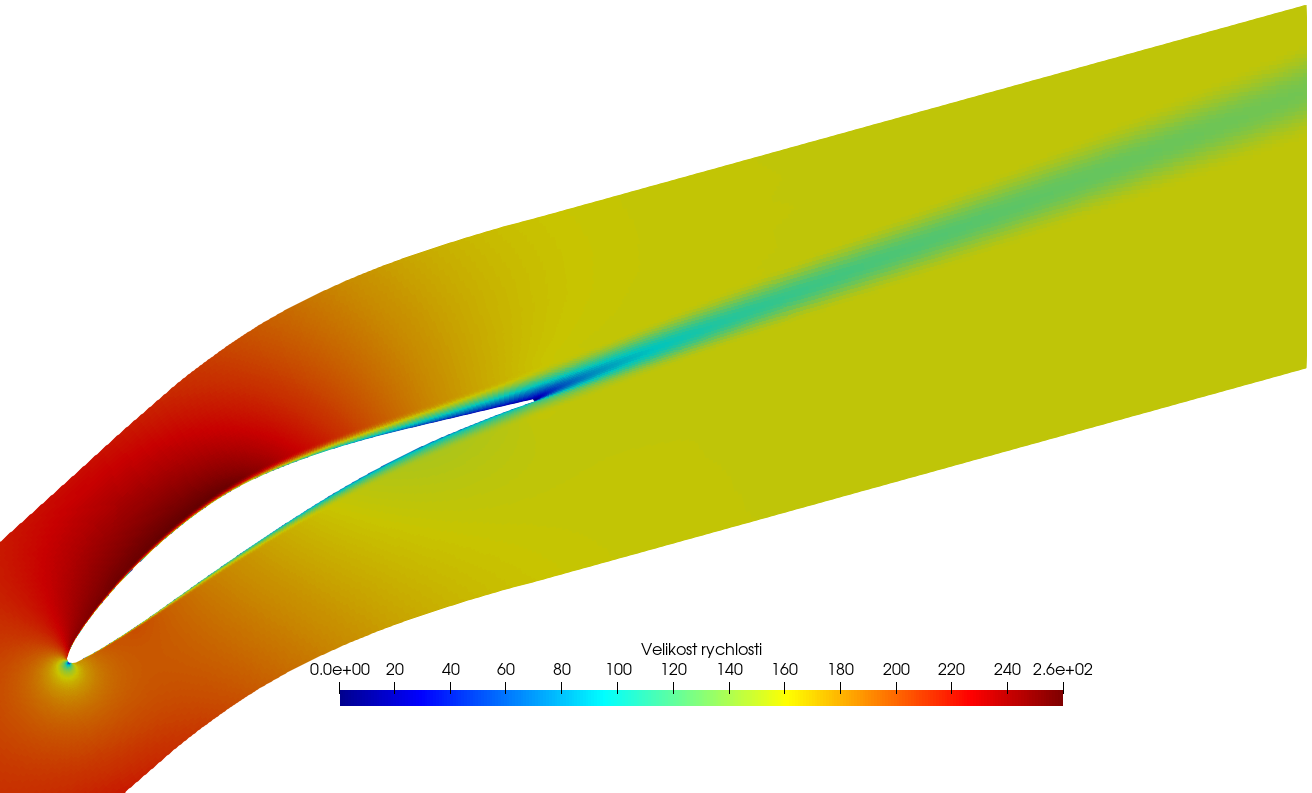
\includegraphics[width=0.7\textwidth]{img/magU_0.png}
	\caption[Velikost rychlosti pro původní lopatku]{Pole velikosti vektoru rychlosti $ ||\mathbf{u}|| $ pro původní profil lopatky.}
	\label{fig:ghs1_U0}
\end{figure}
\begin{figure}[h]
	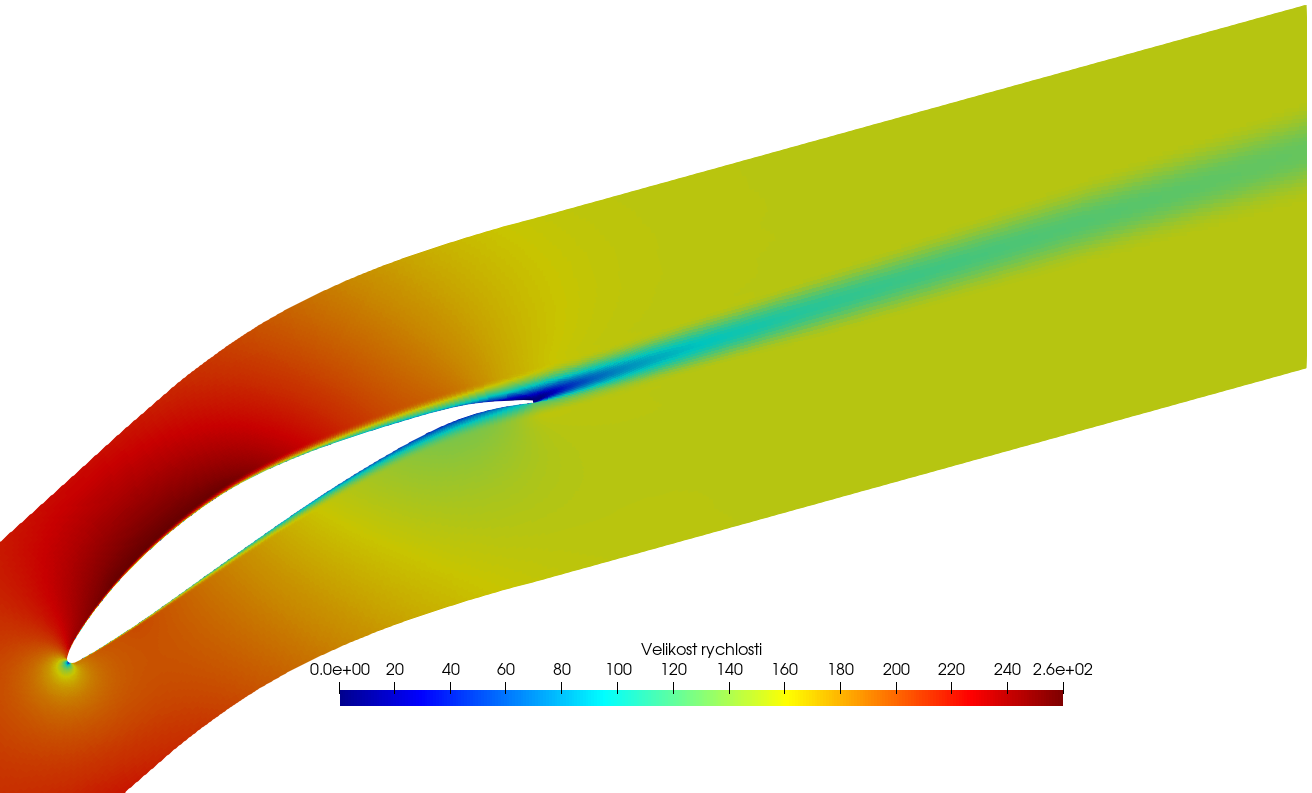
\includegraphics[width=0.7\textwidth]{img/magU_12.png}
	\caption[Velikost rychlosti pro optimalizovanou lopatku]{Pole velikosti vektoru rychlosti $ ||\mathbf{u}|| $ pro optimalizovaný profil lopatky.}
	\label{fig:ghs1_U12}
\end{figure}

Pro detailnější představu o vlivu změny tvaru lopatky je nyní uvedeno několik obrázků.
Nejprve lze porovnat pole velikosti rychlosti pro původní \ref{fig:ghs1_U0} a optimalizovaný \ref{fig:ghs1_U12} tvar lopatky. 
Za koncem lopatky lze vidět pruh nižší velikosti rychlosti, což je úplav. Směr úplavu vizuálně naznačuje směr proudu na výstupu. Při porovnání stavu před a po lze jasně vidět, že směr úplavu změnil. Přesněji se proud ohnul dolů, což odpovídá zmenšení úhlu proudu na výstupu. Zároveň je u optimalizované lopatky vidět větší oblast odtržení proudu u odtokové hrany. Tento efekt potvrzuje i porovnání pole přídavné turbulentní vazkosti $ \nu_t $ na obrázcích \ref{fig:ghs1_nut0} a \ref{fig:ghs1_nut12}. 
\begin{figure}[h]
	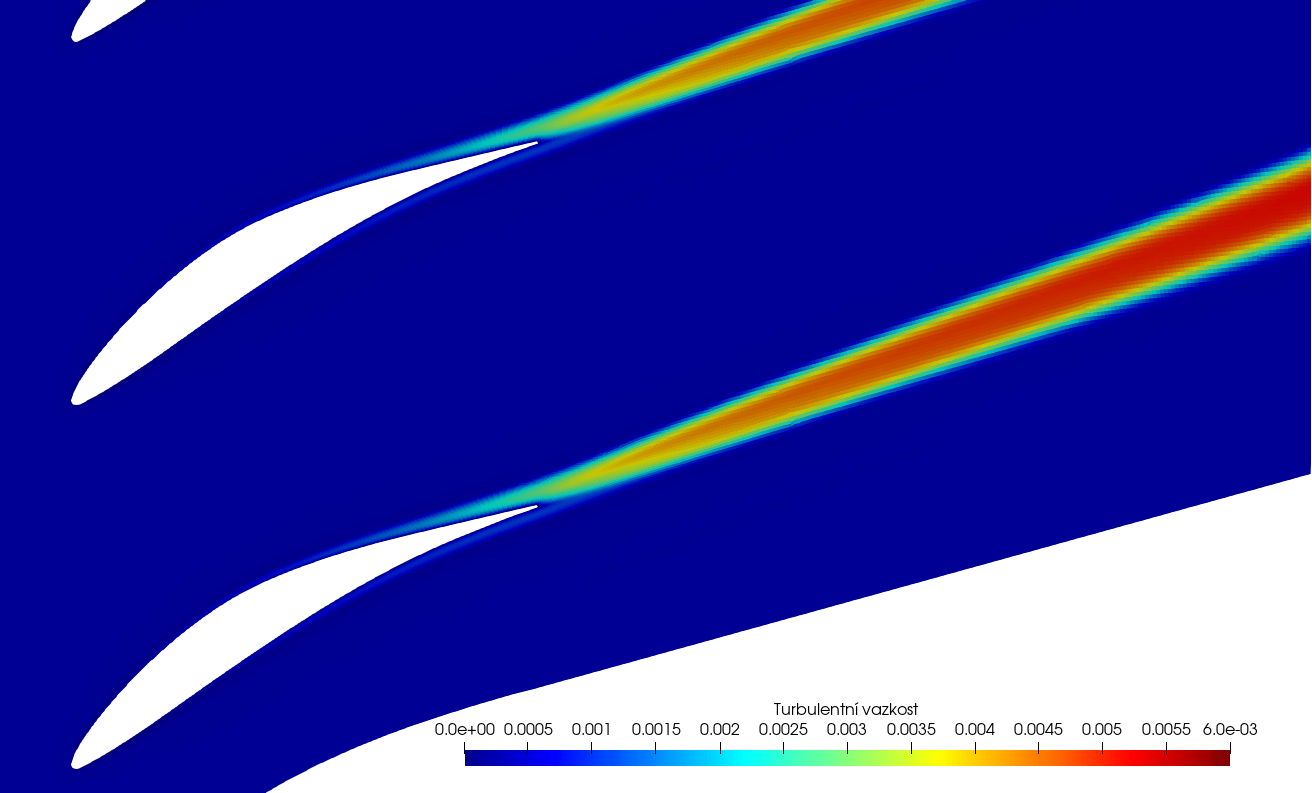
\includegraphics[width=0.7\textwidth]{img/nut_0.png}
	\caption[Turbulentní vazkost pro původní lopatku]{Pole přídavné turbulentní vazkosti $ \nu_t $ pro původní profil lopatky $ \alpha_{2}=\alpha_2^0 $.}
	\label{fig:ghs1_nut0}
\end{figure}
\begin{figure}[h]
	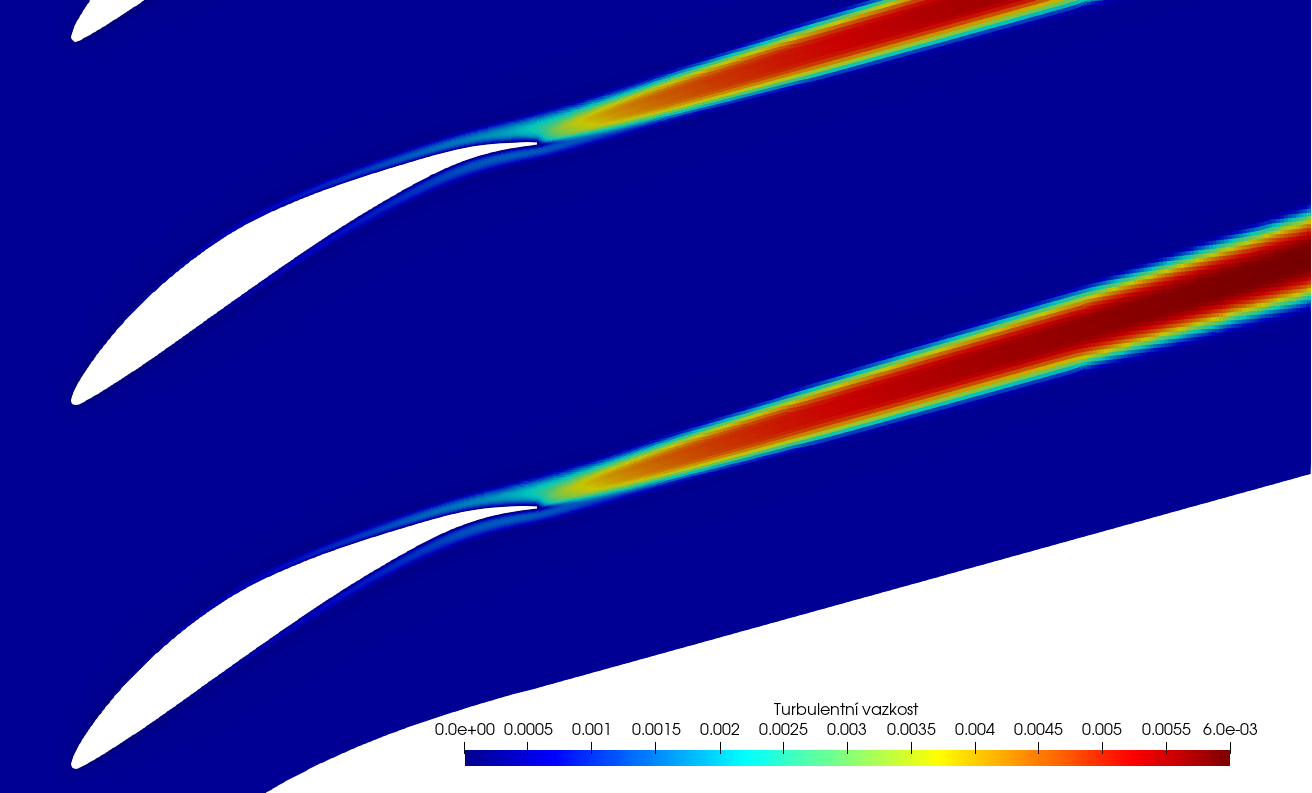
\includegraphics[width=0.7\textwidth]{img/nut_12.png}
	\caption[Turbulentní vazkost pro optimalizovanou lopatku]{Pole přídavné turbulentní vazkosti $ \nu_t $ pro optimalizovaný profil lopatky.}
	\label{fig:ghs1_nut12}
\end{figure}
Maximální velikost přídavné vazkosti v oblasti úplavu za optimalizovanou lopatkou je vyšší a úplav jako takový je širší. To ve výsledku vede na větší ztráty, což dokládá například i zvýšení velikosti síly působící na lopatku ve směru osy $ x $. Optimalizovaná lopatka tedy splňuje cílové ohnutí proudu, z hlediska účinnosti ale tento tvar optimální neníx.
%\begin{figure}
%	\centering
%	\begin{minipage}[t]{0.48\textwidth}
%		\centering
%		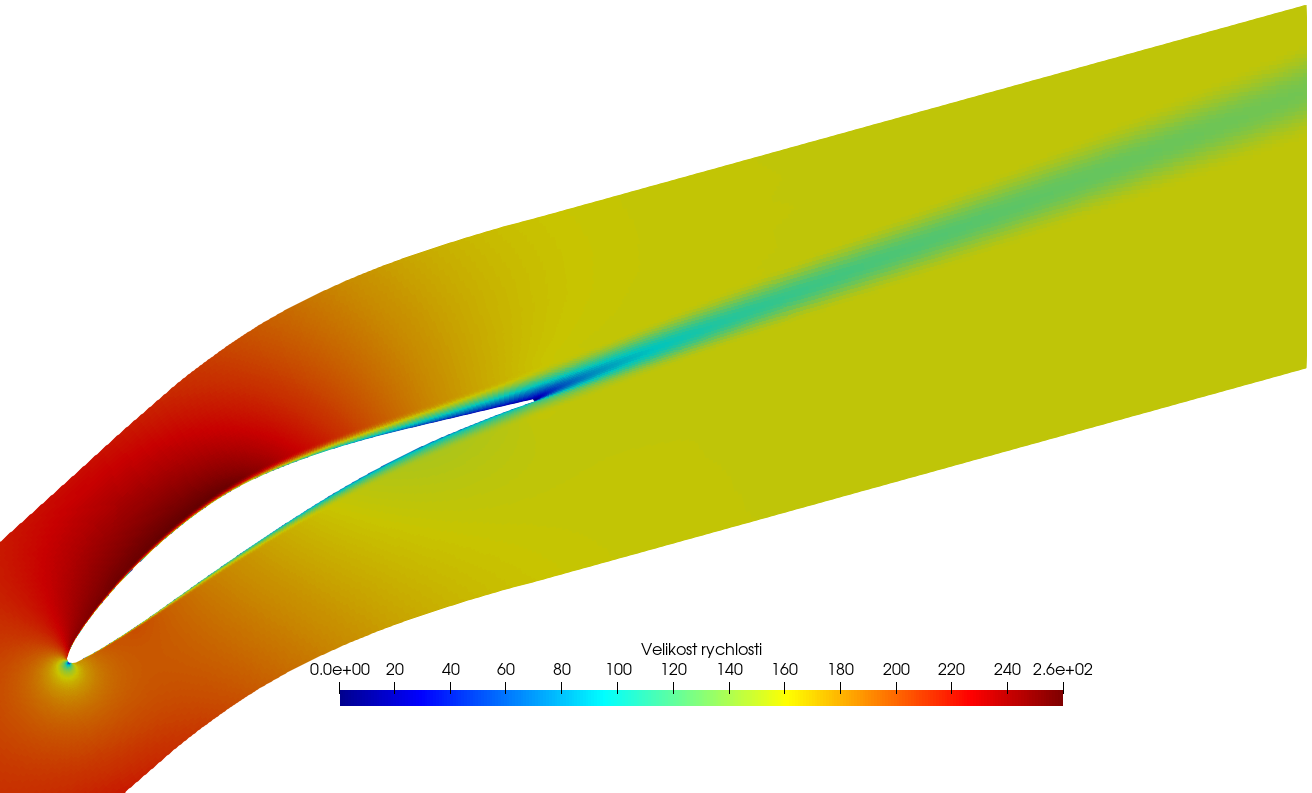
\includegraphics[width=1\textwidth]{img/magU_0.png}
%	\end{minipage}
%	\hfill
%	\begin{minipage}[t]{0.48\textwidth}
%		\centering
%		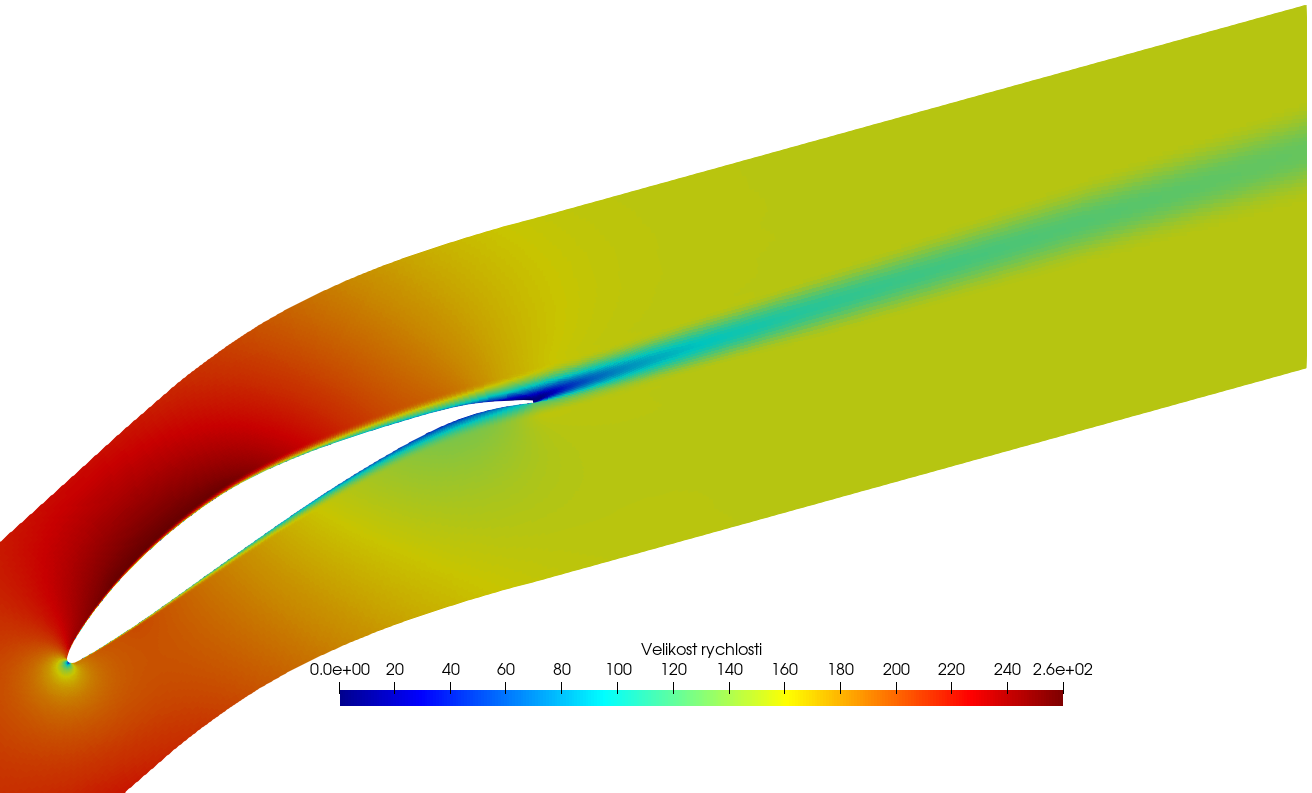
\includegraphics[width=1\textwidth]{img/magU_12.png}
%	\end{minipage}
%	\caption{Pole velikosti vektoru rychlosti pro původní (vlevo) a optimalizovaný (vpravo) profil lopatky.}
%	\label{fig:ghs1_U}
%\end{figure}
%
%\begin{figure}
%\centering
%\begin{minipage}[t]{0.48\textwidth}
%	\centering
%	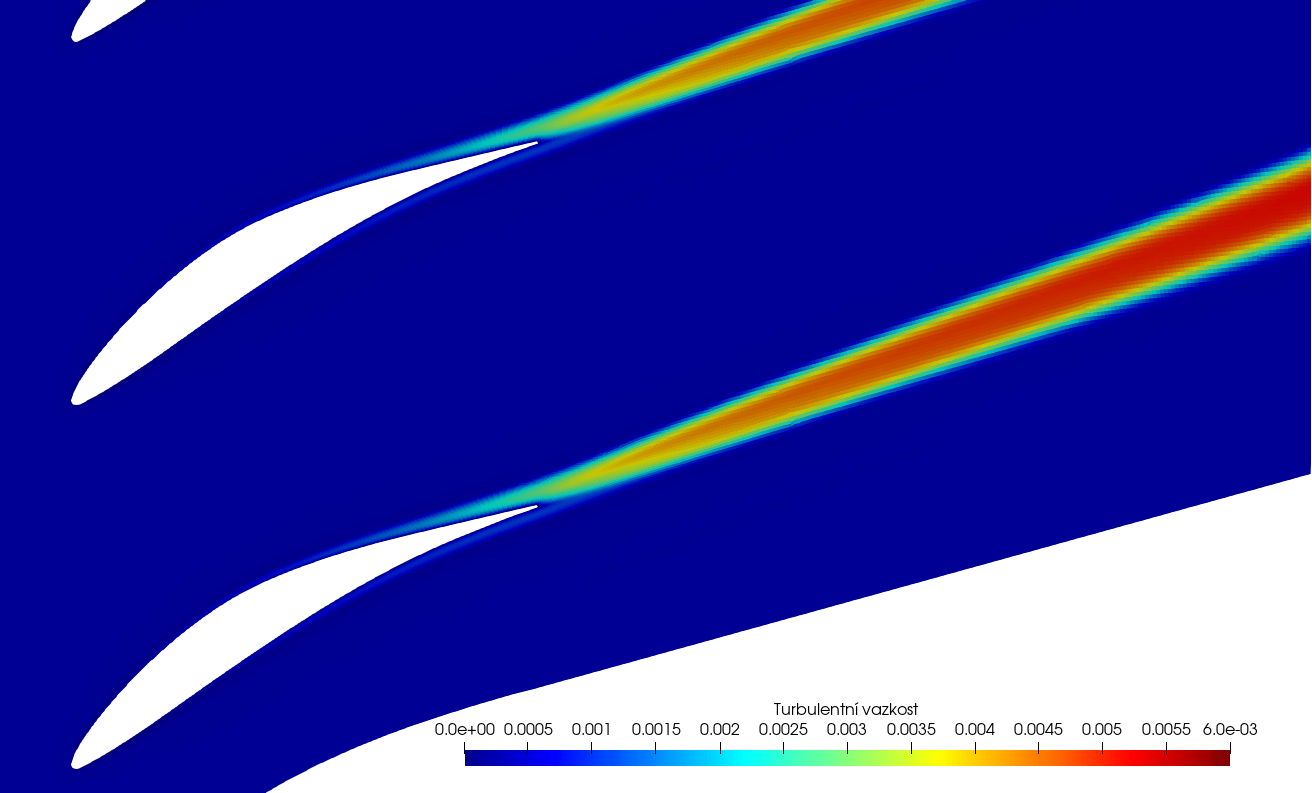
\includegraphics[width=1\textwidth]{img/nut_0.png}
%\end{minipage}
%\hfill
%\begin{minipage}[t]{0.48\textwidth}
%	\centering
%	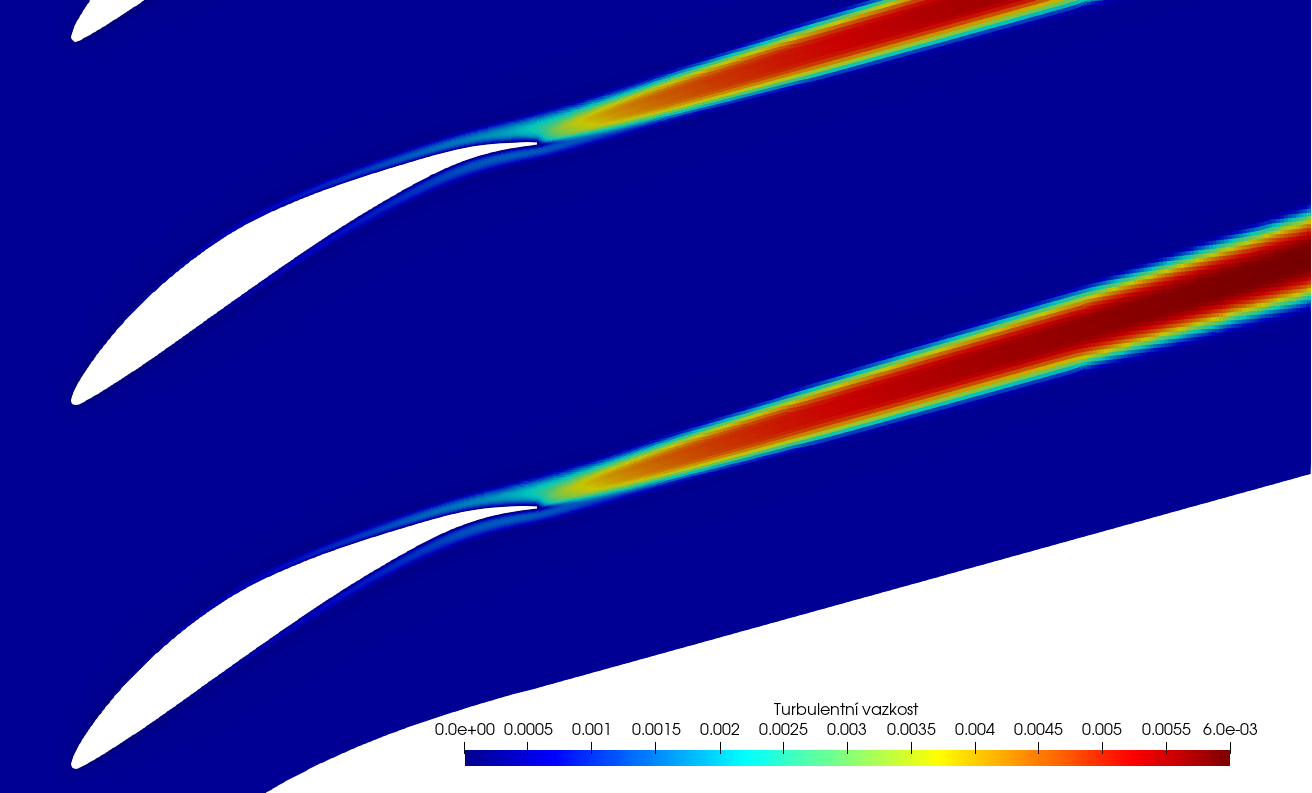
\includegraphics[width=1\textwidth]{img/nut_12.png}
%\end{minipage}
%\caption{Pole přídavné turbulentní vazkosti pro původní (vlevo) a optimalizovaný (vpravo) profil lopatky.}
%\label{fig:ghs1_nut}
%\end{figure}


\subsection{Ověření vhodnějším modelem turbulence}

Pro ověření výsledků optimalizace byl zvolen model $k\text{-}\omega$ SST, který je pro simulace v kompresorech i lopatkových mříží vhodnější než model Spalart-Allmaras. Nejdříve budou ukázány grafy residuí a následně bude podrobněji rozebrán případ $ \Delta \alpha = -4^\circ $.

Pro vyhodnocení residua $ Res_\alpha^{iSST} $ (horní index $ \null^{SST} $ značí vyhodnocení ze simulace s modelem $k\text{-}\omega$ SST) na obrázcích \ref{fig:ghs1_UyAKO} a \ref{fig:ghs1_FyAKO} je na rozdíl od $ Res_\alpha^i $ definovaném rovnicí \ref{eq:res_alpha} použito pro vyhodnocení $ \alpha_{2}^{0SST} $ namísto $ \alpha_{2}^{0} $, tedy
\begin{equation}\label{eq:res_alphaSST}
Res_\alpha^{iSST} = \dfrac{| \alpha_{2}^{iSST}-( \alpha_{2}^{0SST}+\Delta\alpha_2 ) |} {|\alpha_{2}^{0SST}|}.
\end{equation}
Na základě grafů průběhu residua \ref{fig:ghs1_UyAKO} a \ref{fig:ghs1_FyAKO} lze říci, že přestože se v rámci optimalizačního cyklu používá jednodušší model turbulence, tak nový tvar lopatky funguje pro změnu úhlu $ \Delta\alpha\in\langle -2^\circ,+4^\circ\rangle $ i v případě simulace s vhodnějším modelem. Pro větší změny úhlu, konkrétně $ -4^\circ $ a $ +8^\circ $, je ale natočení proudu nesprávné. Pro záporné změny úhlu je tedy předpověď modelu Spalart-Allmaras horší než pro kladné změny úhlu.
Částečné vysvětlení tohoto rozdílu plyne z obrázku \ref{fig:ghs1_sakoUdiff}, který ukazuje relativní rozdíl velikosti rychlosti předpovídané modelem turbulence Spalart-Allmaras ($ \null^{S\text{-}A} $) a $k\text{-}\omega$ SST ($ \null^{SST} $), podle předpisu
\begin{equation}\label{eq:ghs1_sakoUdiff}
\dfrac{||\mathbf{u^{S\text{-}A}||-||u^{SST}}||}{||\mathbf{u_1}||}.
\end{equation}
Největší rozdíl je v blízkosti odtokové hrany na podtlakové straně, kde dochází k odtržení proudu. Simulace s modelem Spalart-Allmaras zde předpovídá mnohem větší velikost rychlosti a lze tedy usoudit, že nezachycuje odtržení správným způsobem. Z obrázku \ref{fig:ghs1_sakoUdiff} je mimo jiné vidět, že výpočet s modelem $k\text{-}\omega$ SST předpovídá, že změna úhlu proudu bude větší než žádané 4°. Z grafu průběhu residua předtím nešlo říct, jestli je podle $k\text{-}\omega$ SST ohnutí proudu větší či menší, protože rozdíl v čitateli je v absolutní hodnotě.
\begin{figure}[H]
	\centering
	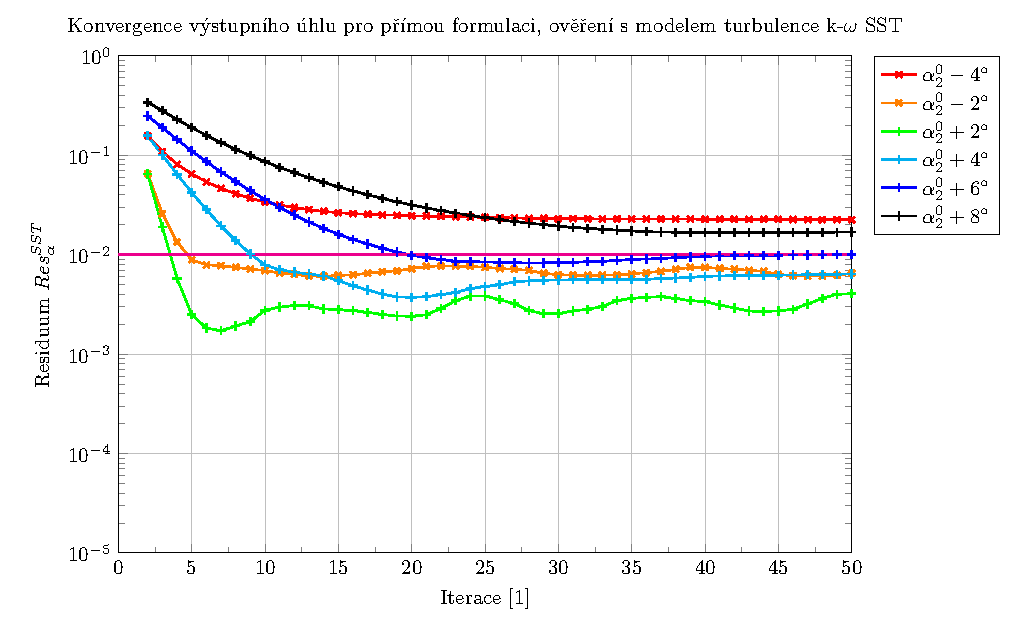
\includegraphics[width=0.95\textwidth]{img/UyAKO.pdf}
	\caption[ Průběh residua $ Res_{\alpha}^{iSST} $, přímá formulace, $k\text{-}\omega$ SST ]{Průběh residua $ Res_{\alpha}^{iSST} $ \ref{eq:res_alpha} pro přímou formulaci cílové funkce $ J $ v průběhu iteračních cyklů. Hranice optimálního řešení $ 1\% $ je naznačena růžovou čarou. Výpočty používají model turbulence $k\text{-}\omega$ SST.}
	\label{fig:ghs1_UyAKO}
\end{figure}
\begin{figure}[H]
	\centering
	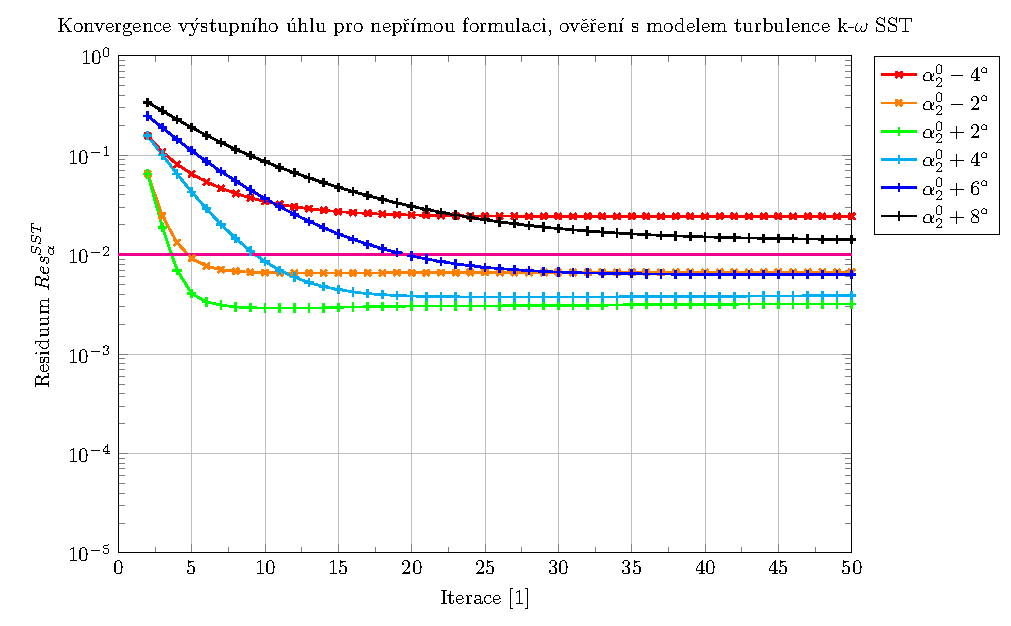
\includegraphics[width=0.95\textwidth]{img/FyAKO.pdf}
	\caption[ Průběh residua $ Res_{\alpha}^{iSST} $, nepřímá formulace, $k\text{-}\omega$ SST ]{Průběh residua $ Res_{\alpha}^{iSST} $ \ref{eq:res_alpha} pro nepřímou formulaci cílové funkce $ J $ v průběhu iteračních cyklů. Hranice optimálního řešení $ 1\% $ je naznačena růžovou čarou. Výpočty používají model turbulence $k\text{-}\omega$ SST.}
	\label{fig:ghs1_FyAKO}
\end{figure}
\begin{figure}[H]
\centering
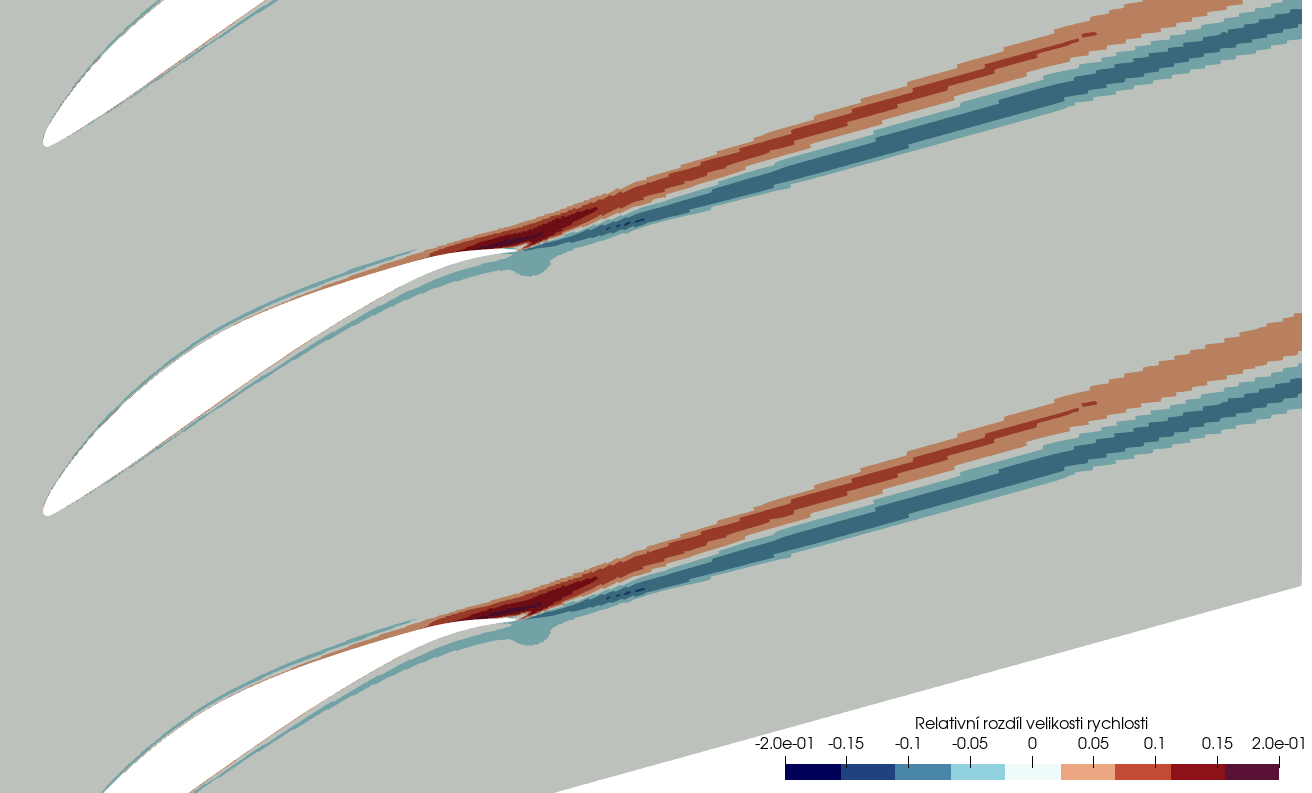
\includegraphics[width=0.95\textwidth]{img/sako_magUdiff.png}
\caption[Rozdíl rychlosti pro modely turbulence]{
Rozdíl velikosti rychlosti pro simulaci s modelem Spalart-Allmaras a s modeleme $k\text{-}\omega$ SST. V červené oblasti předpovídá simulace $ \null^{S\text{-}A} $ vyšší velikost rychlosti, v modré oblasti pak menší, než simulace $ ^{SST} $.}
\label{fig:ghs1_sakoUdiff}
\end{figure}










\chapter{Závěr}
\lipsum[1]
 




%\blindmathtrue
%\blinddocument

%\begin{table}
%\begin{ctucolortab}
%\begin{tabular}{cc}
%\bfseries Foo & \bfseries Bar \\\Midrule
%foo1 & bar1 \\
%foo2 & bar2
%\end{tabular}
%\end{ctucolortab}
%\caption{Foobar.}
%\label{tab:foobar}
%\end{table}

%\begin{figure}
%
\includegraphics[width=0.4\textwidth]{ctu_logo_black}
%\caption{Black logo of the CTU in Pragueueue.}
%\end{figure}

%\begin{figure}[!t]
%
\includegraphics[width=0.4\textwidth]{ctu_logo_blue}
%\caption{Blue logo of the CTU in Pragueueue.}
%\end{figure}



\appendix

\printnomenclature

\printindex

\bibliographystyle{abbrv}
\bibliography{bibliography/_main}



\end{document}